\section{Introduction}

Before we can discuss the results from our more technical research in Chapters \ref{chap:resistive_phase_mixed_alfven_waves} and \ref{chap:resonant_absorption_in_an_oblique_field} we need to first understand the dynamics of waves in a more simple domain.
This chapter models footpoint driven linear Alfv\'en waves in a uniform domain to establish some of the key ideas we will use throughout this thesis.
We will see in Chapter \ref{chap:resistive_phase_mixed_alfven_waves} that if an invariant direction is assumed, in this case, $\pdv*{}{y}=0$, then the velocity perturbations in the invariant direction (in this case, $v_y$), must satisfy the Alfv\'en wave equation. Chapter \ref{chap:resonant_absorption_in_an_oblique_field} shows that propagating fast waves with a given frequency will mode convert at a field line with the same natural frequency to form standing Alfv\'en waves. This phenomenon is called resonant absorption. Moreover, a similar effect was demonstrated in more general three-dimensional domains (see for example, \citealt{Wright2016,Elsden2017,Elsden2018}). This suggests that Alfv\'en waves and approximate Alfv\'en waves are ubiquitous throughout the solar atmosphere.

The outline of this chapter is as follows. 
In Section \ref{sec:chap_2_model_and_equations} we introduce the model we use and discuss the assumptions we will make. In Sections \ref{sec:chap_2_closed_loop_general_soln}-\ref{sec:closed_loop_sinusoidal_solution} we calculate the solution for a closed loop with a footpoint driver. We show how a footpoint driver can excite resonances along the loop. We will calculate the solutions for the case where the driver is sinusoidal and excites resonant frequencies, nearly resonant frequencies and frequencies halfway in between different resonant frequencies.
After that, in Section \ref{sec:closed_loop_random_driver}, we will study the solution when we use a noisy driver. We think of a noisy driver as a superposition of an infinite number of sinusoidal drivers. We use a white and red noise force driver where the slope of its power spectrum defines the noise's colour, and this is explained further in Section \ref{sec:closed_loop_random_driver}. One of the goals in this section is to determine if the randomly driven loop's energy will grow to infinity or oscillate about a finite value. 
In Section \ref{sec:leaky_loop_reflection_coefficent}-\ref{sec:leaky_loop_steady_state_solution} we consider the case where waves can leak out of the loop. To estimate the transition region's reflection coefficient, we approximate the corona and chromosphere using a similar model to that used in \citet{Hollweg1984b}. In Section \ref{sec:leaky_loop_steady_state_solution}, we show that leakage prevents the energy from growing to infinity, even if a natural frequency is excited. We show that the system tends towards a state where the whole system oscillates at the driver frequency, called the steady-state solution. Finally, Section \ref{sec:phase_mixing} introduces phase mixing to show some of the key results which are used in Chapter \ref{chap:resistive_phase_mixed_alfven_waves}.

% To begin with, we will look at Alfv\'en waves on a single field line. After that, we will discuss the behaviour in an ideal medium. After that, we will analyse the effects of introducing resistivity and viscosity to the system, making the system non-ideal. We will look at how a mechanism called phase-mixing can enhance the rate at which wave-energy is dissipated. Finally, we will assess the viability of linear phase-mixed Alfv\'en waves in straight loops as a coronal heating mechanism.

\section{Model and equations}
\label{sec:chap_2_model_and_equations}

In this chapter, we will model perturbations on a background medium. We will make the same assumption as described by Equations \eqref{eq:linear_assumotion_v}-\eqref{eq:linear_assumotion_rho}, namely, that we will model linear perturbations on a static background medium. We assume the perturbations' velocity amplitude satisfies the Alfv\'en wave equation, see Equation \eqref{eq:alfven_wave_equation}. We model the domain as ideal, which means we neglect resistivity and viscosity. Like with Section \ref{sec:mhd_waves_dispersion_relation} we will model the background quantities as uniform. In reality, the coronal field is non-uniform, and the density is stratified due to gravity. The propagation of Alfv\'en waves through a divergent and stratified coronal structure is investigated in, for example, \citet{Smith2007}. The effects of loop curvature on coronal kink oscillations are investigated in, for example, \citet{vanDoorsselaere2009}. In the next chapter, we will study waves in a domain where the background density has a transverse density profile. Modelling the background quantities as uniform means the background field must be straight. Without loss of generality, we model the background field, $\vec{B}_0$, as
\begin{equation}
    \tag{\ref{eq:background_field}}
    \vec{B}_0 = B_0\vec{\hat{z}}.
\end{equation}

In Section \ref{sec:mhd_waves_dispersion_relation} we showed that with these assumptions and assuming $\beta=0$, two types of solutions exist, namely fast and Alfv\'en waves. In this chapter we choose only to investigate Alfv\'en waves, i.e. waves with a velocity amplitude $\vec{u}$ which satisfies
\begin{equation}
    \label{eq:alfven_wave_equation2}
    \mathcal{L}\vec{u}=\qty(\pdv[2]{}{t}+v_{A0}^2\pdv[2]{}{z})\vec{u}=0,
\end{equation}
where $\mathcal{L}$ is given by Equation \eqref{eq:alfven_wave_equation_operator}.
Let
\begin{gather}
    \label{eq:y_component_of_u}
     \vec{u}(z,t) = u(z,t)\vec{\hat{y}}, \\
     \label{eq:y_component_of_b}
     \vec{b}(z,t) = b(z,t)\vec{\hat{y}}.
\end{gather}

We choose our domain to be given by
\[z\in[-l_z,l_z],\]
where
\[L_z=2l_z,\]
gives the length of the loop. To begin with, we impose line-tied boundary conditions at the ends of the loop, i.e.
\begin{equation}
    \label{eq:bcs_chap_2}
    u(-l_z,t) = f_{driv}(t),\quad u(l_z,t)=0,
\end{equation}
however, in Section \ref{sec:leaky_loop_general_solution} we consider a partially confined loop. Additionally, we impose the following initial condition
\begin{equation}
    \label{eq:initial_condition}
    u(z,0) = 0,\ \left.\pdv{u}{t}\right|_{t=0} = 0,\ \text{for}\ z\ne-l_z
\end{equation}
Without loss of generality, we impose the driver at only the bottom boundary. We do not lose generality because the system is linear and is symmetric about $z=0$. Therefore, we can construct a general solution by superimposing solutions with the driver imposed at only one of the boundaries. We impose zero velocity at $z=l_z$; in other words, we impose line-tied boundary conditions. The chromosphere and photosphere are orders of magnitude denser than the corona (see Figure \ref{fig:VAL_atmosphere}) over a length scale of just a few Mm, this means that the amplitude of waves propagating from the corona to the chromosphere and photosphere typically reduces significantly. Line-tied ($\vec{u}=0$) boundary conditions are convenient to simulate this behaviour. We approximate the transmission and reflection coefficients in Section \ref{sec:leaky_loop_reflection_coefficent}.

\section{Closed loop: general solution}
\label{sec:chap_2_closed_loop_general_soln}

In this section, we will construct the general solution to Equation \eqref{eq:alfven_wave_equation2} with boundary and initial conditions described by Equation \eqref{eq:bcs_chap_2} and \eqref{eq:initial_condition}. We will construct this solution step-by step via a method of images approach. By d'Alambert's formula we can write solutions to the 1D wave equation, Equation \eqref{eq:alfven_wave_equation2}, as
\begin{equation}
    u(z,t) = F\qty(t - \frac{z}{v_{A0}}) + G\qty(t + \frac{z}{v_{A0}}).
\end{equation}
Consider for now the case where the top boundary is open, and we impose the condition that only waves propagating in the positive $z$ direction can exist. Hence, a valid solution is nearly given by
\[u(z,t) = f_{driv}\qty(t - \frac{z+l_z}{v_{A0}}).\]
however, this does not satisfy our initial condition. We need $u$ and $\pdv*{u}{t}$ to be initially equal to zero for $z>-l_z$. A solution which satisfies the initial condition is given by
\[u(z,t) = f_{driv}\qty(t - \frac{z+l_z}{v_{A0}})H\qty(t - \frac{z+l_z}{v_{A0}}),\]
where $H(x)$ is the Heaviside step function.

Note that the line-tied boundary condition, $u(l_z,t)$, causes any waves propagating in the positive $z$-direction to reflect at $z=l_z$. We can simulate this reflection by allowing the real wave to leave the domain and introducing a `ghost' wave that propagates in the negative $z$-direction. The superposition of the domain wave and `ghost' wave cancels to give zero. Therefore, a solution which reflects at $z=l_z$ is given by
\[u(z,t) = f_{driv}\qty(t - \frac{z+l_z}{v_{A0}})H\qty(t - \frac{z+l_z}{v_{A0}}) - f_{driv}\qty(t + \frac{z-3l_z}{v_{A0}})H\qty(t + \frac{z-3l_z}{v_{A0}}).\]
Unfortunately, this solution does not in general satisfy $u(-l_z,t)=f_{driv}(t)$. We need waves propagating in the negative $z$-direction to reflect at the $z=-l_z$ boundary. We need waves to reflect back and forth forever between $z=-l_z$ and $z=l_z$. This means we need an infinite number of `ghost' waves to simulate reflection an infinite number of times. A solution which satisfies this condition is given by
\begin{equation}
    \label{eq:closed_loop_general_solution_infinit}
    u(z,t) = \sum_{k=0}^\infty(-1)^kH(\theta_k)f_{driv}(\theta_k),
\end{equation}
where
\begin{equation}
    \label{eq:theta_k}
    \theta_k=t-(-1)^k\frac{z}{v_{A0}}-\frac{(2k+1)l}{v_{A0}}.
\end{equation}
This equation is a valid solution to our problem. However, we can simplify it further. Note that the $k$'th term in the series only enters the domain after $k$ reflections have occurred. Therefore, if $t$ is finite, only a limited number of terms in the series are needed. Note that each reflection occurs at times
\begin{equation}
    t = \frac{n L_z}{v_{A0}},
\end{equation}
where $n\in\mathds{N}$. Therefore, at time $t$ the number of reflections which have occurred, $m$, is given by
\begin{equation}
    \label{eq:m}
    m = \left\lfloor\frac{t v_{A0}}{L_z}\right\rfloor,
\end{equation}
where $\lfloor \rfloor$ denotes the floor function which rounds the input down to the nearest integer. Hence, we can simplify Equation \eqref{eq:closed_loop_general_solution_infinit} to give
\begin{equation}
    \label{eq:closed_loop_general_solution_finite}
    \begin{aligned}
    u(z,t) &= \sum_{k=0}^m(-1)^kH(\theta_k)f_{driv}(\theta_k) \\
    &= \sum_{k=0}^{m-1}(-1)^kf_{driv}(\theta_k) + (-1)^mH(\theta_m)f_{driv}(\theta_m).
    \end{aligned}
\end{equation}
To see that more clearly that Equation \eqref{eq:closed_loop_general_solution_finite} is indeed a valid solution satisfying our boundary conditions consider the following. We know that each term satisfies the wave equation as they are of the form given by D'Alambert's formula. We can check $u$ does indeed equal 0 at $z=l_z$ and $u=f_{driv}(t)$ at the $z=-l_z$ either numerically or analytically.

\section{Closed loop: sinusoidal solution}
\label{sec:closed_loop_sinusoidal_solution}

Equation \eqref{eq:closed_loop_general_solution_finite} gives the solution for a general driver, $f_{driv}$. In this section, we investigate the solution for the case where
\begin{equation}
    \label{eq:driver_sinusoidal}
    f_{driv}(t)=u_0\exp(i\omega t).
\end{equation}
Substituting Equation \eqref{eq:driver_sinusoidal} into Equation \eqref{eq:closed_loop_general_solution_finite} gives
\begin{equation}
    \label{eq:u_sinusoidal_driver}
    \begin{aligned}
    u(z,t) = u_0\sum_{k=0}^{m}(-1)^kH(\theta_k)\exp(i\omega\theta_k).
    \end{aligned}
\end{equation}
From Equation \eqref{eq:by_eqn_linear} we can infer that
\begin{equation}
    \label{eq:b_in_terms_of_u}
    i\omega b = B_0\pdv{u}{z}.
\end{equation}
Note that
\[\pdv{\theta_k}{z}=-\frac{(-1)^k}{v_{A0}},\]
therefore, substituting Equation \eqref{eq:u_sinusoidal_driver} into Equation \eqref{eq:b_in_terms_of_u} gives
\begin{equation}
    b = -\frac{B_0u_0}{v_{A0}}\sum_{k=0}^{m}H(\theta_k)\exp(i\omega\theta_k).
\end{equation}

The equations above describe the solution for all $z$ and $t$. Section \ref{sec:soln_at_z=0} uses the geometric series formula to simplify the above series. We see that the time evolution can vary significantly depending on the driver frequency, $\omega$.

\subsection{Solution at \texorpdfstring{$z=0$}{z=0}}
\label{sec:soln_at_z=0}

Note that the wave-front reaches $z=0$ at times
\begin{equation}
    t = \qty(n+\frac{1}{2})\frac{L_z}{v_{A0}},
\end{equation}
for $n\in\mathds{N}$. Therefore, the number of times the wave-front has reached $z=0$ is given by $m'+1$ where
\begin{equation}
    m'=\left\lfloor\frac{tv_{A0}}{L_z}-\frac{1}{2}\right\rfloor.
\end{equation}
Hence,
\begin{equation}
    \begin{aligned}
    u(0,t) &= u_0\sum_{k=0}^{m'}(-1)^k\exp(i\omega\theta_k) \\
    &= u_0\exp[i\omega(t - l_z/v_{A0})]\sum_{k=0}^{m'}(-1)^k\exp(-2ik\omega l_z/ v_{A0}).
    \end{aligned}
\end{equation}
Let
\begin{equation}
    r = \exp(-2i\omega l_z/ v_{A0}).
\end{equation}
Therefore, for $r\ne-1$, using the formula for the geometric series, the above series can be simplified as
\begin{equation}
    \label{eq:u0_non_res}
    \begin{aligned}
    u(0,t) &= u_0\exp[i\omega(t - l_z/v_{A0})]\sum_{k=0}^{m'}(-r)^k \\
    &= u_0\exp[i\omega(t - l_z/v_{A0})]\frac{1-(-r)^{m'+1}}{1+r}.
    \end{aligned}   
\end{equation}
If $r=-1$ then 
\begin{equation}
    \label{eq:u0_odd_harmonic}
    \begin{aligned}
    u(0,t) = u_0\exp[i\omega(t - l_z/v_{A0})](m'+1).
    \end{aligned}   
\end{equation}

Hence, for $r\ne1$
\begin{equation}
    \begin{aligned}
    b(0,t)&=-\frac{B_0u_0}{v_{A0}}\exp[i\omega(t - l_z/v_{A0})]\sum_{k=0}^{m'}\exp(-2ik\omega l_z/ v_{A0}) \\
    &=-\frac{B_0u_0}{v_{A0}}\exp[i\omega(t - l_z/v_{A0})]\frac{1-r^{m'+1}}{1-r}.
    \end{aligned},
\end{equation}
and for $r=1$,
\begin{equation}
    \label{eq:b0_even_harmonic}
    b(0,t)=-\frac{B_0u_0}{v_{A0}}\exp[i\omega(t - l_z/v_{A0})](1+m').
\end{equation}

For $r\ne-1$, the absolute value of $u(0,t)$ is given by
\begin{equation}
    \abs{u(0,t)}=u_0
    \begin{cases}
    \abs{\sin\{(m'+1)\omega l_z/v_{A0}\}/\cos(\omega l_z/v_{A0})}, &\text{for}\ m'+1\ \text{even}, \\
    \abs{\cos\{(m'+1)\omega l_z/v_{A0}\}/\cos(\omega l_z/v_{A0})}, &\text{for}\ m'+1\ \text{odd}, \\
    \end{cases}
\end{equation}
which is equivalent to
\begin{equation}
    \label{eq:abs_u0_non_res}
    \abs{u(0,t)}=u_0\abs{\frac{\sin\{(m'+1)(\omega l_z/v_{A0}+\pi/2)\}}{\cos(\omega l_z/v_{A0})}}.
\end{equation}
For $r=-1$
\begin{equation}
     \abs{u(0,t)}=u_0(m'+1).
\end{equation}

For $r\ne-1$, the absolute value of $b(0,t)$ is given by
\begin{equation}
    \label{eq:abs_b0_non_res}
    \abs{b(0,t)}=\frac{u_0 B_0}{v_{A0}}\abs{\frac{\sin\{(m'+1)\omega l_z/v_{A0}\}}{\sin(\omega l_z/v_{A0})}}.
\end{equation}
For $r=-1$
\begin{equation}
    \label{eq:abs_b0_res}
    |b(0,t)|=\frac{B_0 u_0}{v_{A0}}(m'+1).
\end{equation}

We call $\omega_n$ for $n\in \mathds{Z}$ the resonant frequencies which satisfy
\begin{gather}
    \frac{\omega_n l_z}{v_{A0}}=\frac{n\pi}{2}, \\
    \label{eq:chap_2_omega_n}
    \implies \omega_n = \frac{n\pi v_{A0}}{L_z}.
\end{gather}
Equations \eqref{eq:abs_u0_non_res}-\eqref{eq:abs_b0_res} show that for $\omega\ne\omega_n,$
the solutions oscillate about a finite value, but for $\omega=\omega_n,$
then either $u$ or $b$ at the loop apex grows linearly with time. In Sections \ref{sec:case_where_omega=omega_n}-\ref{sec:case_where_omega_ne_omega_n} we investigate the solutions for the cases where $\omega=\omega_n$, $\omega\approx\omega_n$ and $\omega\ne\omega_n$, where $\omega_\ne \omega_n$ is the case where the driver frequency is as far away from the resonant frequencies as possible.

\subsection{Resonant case}
\label{sec:case_where_omega=omega_n}

In this section, we investigate solutions for the case where $\omega=\omega_n$. If $n$ is odd, then we say the odd harmonic has been excited, if $n$ is even then we say an even harmonic has been excited. 

Note that
\begin{equation}
    \label{eq:u0_odd__even_harmonic}
    u(0,t) = u_0 \exp[i\omega_n(t - l_z/v_{A0})]\begin{cases}
   (m'+1), & n\ \text{odd}, \\
   [1-(-1)^{m'+1}]/2, & n\ \text{even}.
    \end{cases}
\end{equation}
\begin{equation}
    \label{eq:b0_odd__even_harmonic}
    b(0,t) = -\frac{B_0u_0}{v_{A0}} \exp[i\omega_n(t - l_z/v_{A0})]\begin{cases}
   [1-(-1)^{m'+1}]/2, & n\ \text{odd}, \\
   (m'+1), & n\ \text{even}.
    \end{cases}
\end{equation}
The Poytning flux at $z=0$, directed in the $z$-direction, $S_{z0}$, is given by
\begin{equation}
    S_{z0} = \vec{S}\cdot\vec{\hat{z}}|_{z=0}.
\end{equation}
Since, $\vec{u}=0$
Hence, using  Equation \eqref{eq:poynting_flux_linear}, $S_{z0}$ is given by
\begin{equation}
    S_{z0} = -\frac{B_0}{\mu}\Im[u(0,t)]\Im[b(0,t)],
\end{equation}
where $\Im[\,]$ returns the imaginary component of the input. Using the divergence theorem, and the fact that $\vec{u}=0$ at $z=l_z$, we know that $-S_{z0}$ gives the rate of change of energy in the top half the loop. Using Equations \eqref{eq:u0_odd__even_harmonic} and \eqref{eq:b0_odd__even_harmonic} we can show that $-S_{z0}$ is given by
\begin{equation}
    -S_{z0}=-\frac{B_0u_0^2}{2\mu v_{A0}}\sin^2[\omega_n(t - l_z/v_{A0})](m'+1)(1-(-1)^{m'+1}).
\end{equation}

\begin{figure}
    \centering
    \vspace{-20pt}
    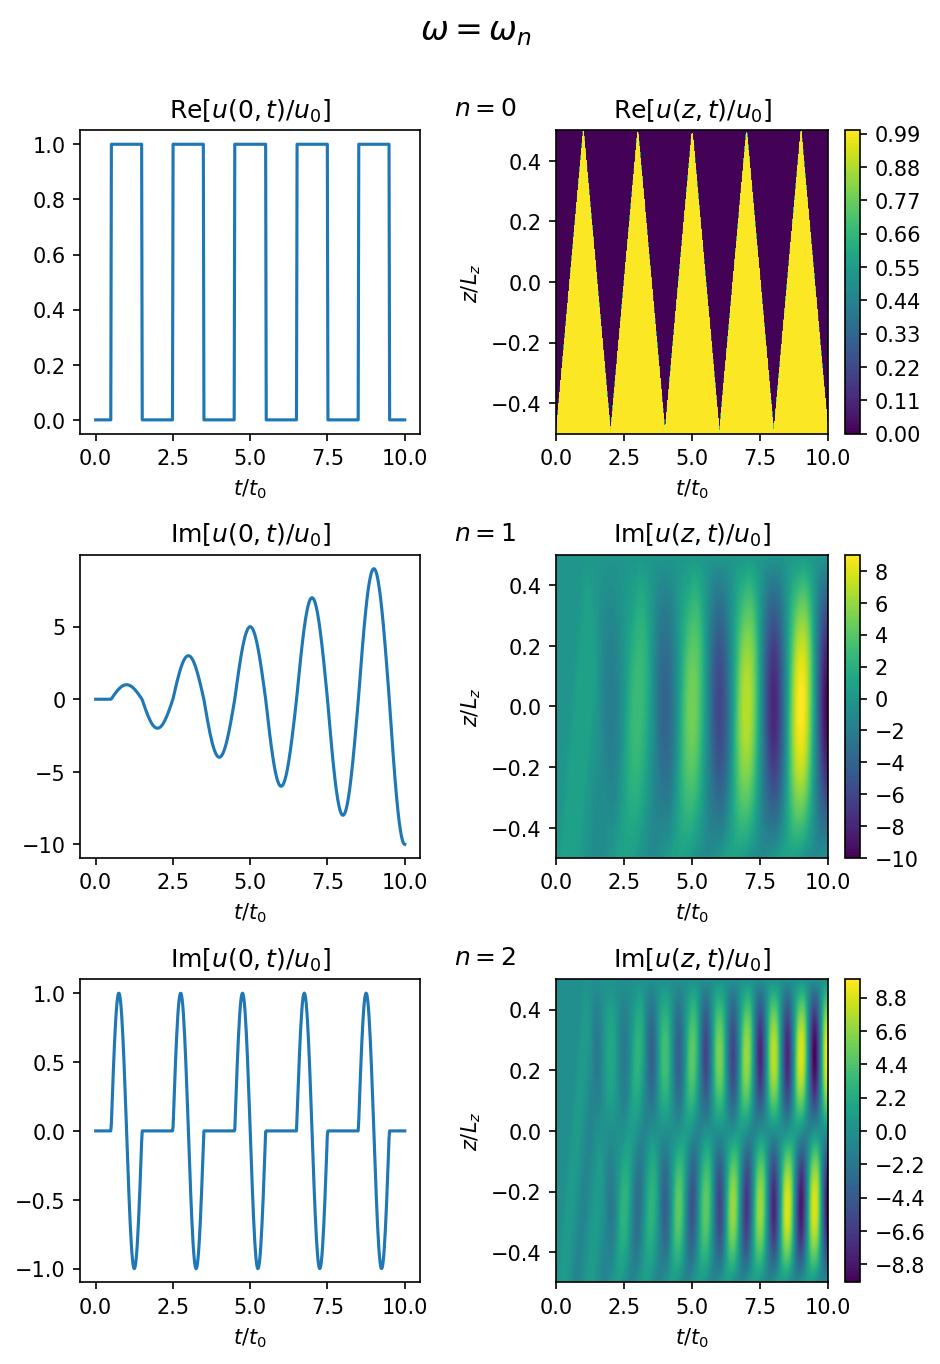
\includegraphics[width=\textwidth,height=0.85\textheight,keepaspectratio]{figures/chapter02/case_where_omega=omega_n_u.png}
    \vspace{-10pt}
    \caption{This figure shows contour plots of the velocity, $u$, and line plots at $z=0$. The driver frequency is given by $\omega=\omega_n$. Each row shows the solution for different values of $n$. The top row shows the real part and the other rows show the imaginary part. The normalising constant, $t_0$, is given by Equation \eqref{eq:t0}. The code used to make this figure is available on GitHub in the following directory:\newline
    \href{https://github.com/aleksyprok/apkp_thesis/blob/main/Python/Chapter2/case_where_omega\%3Domega_n.py}{$\rightarrow$ Python/Chapter2/case\_where\_omega=omega\_n.py}
    }
    \label{fig:case_where_omega=omega_n_u}
    \vspace{-30pt}
\end{figure}

\begin{figure}
    \centering
    \vspace{-20pt}
    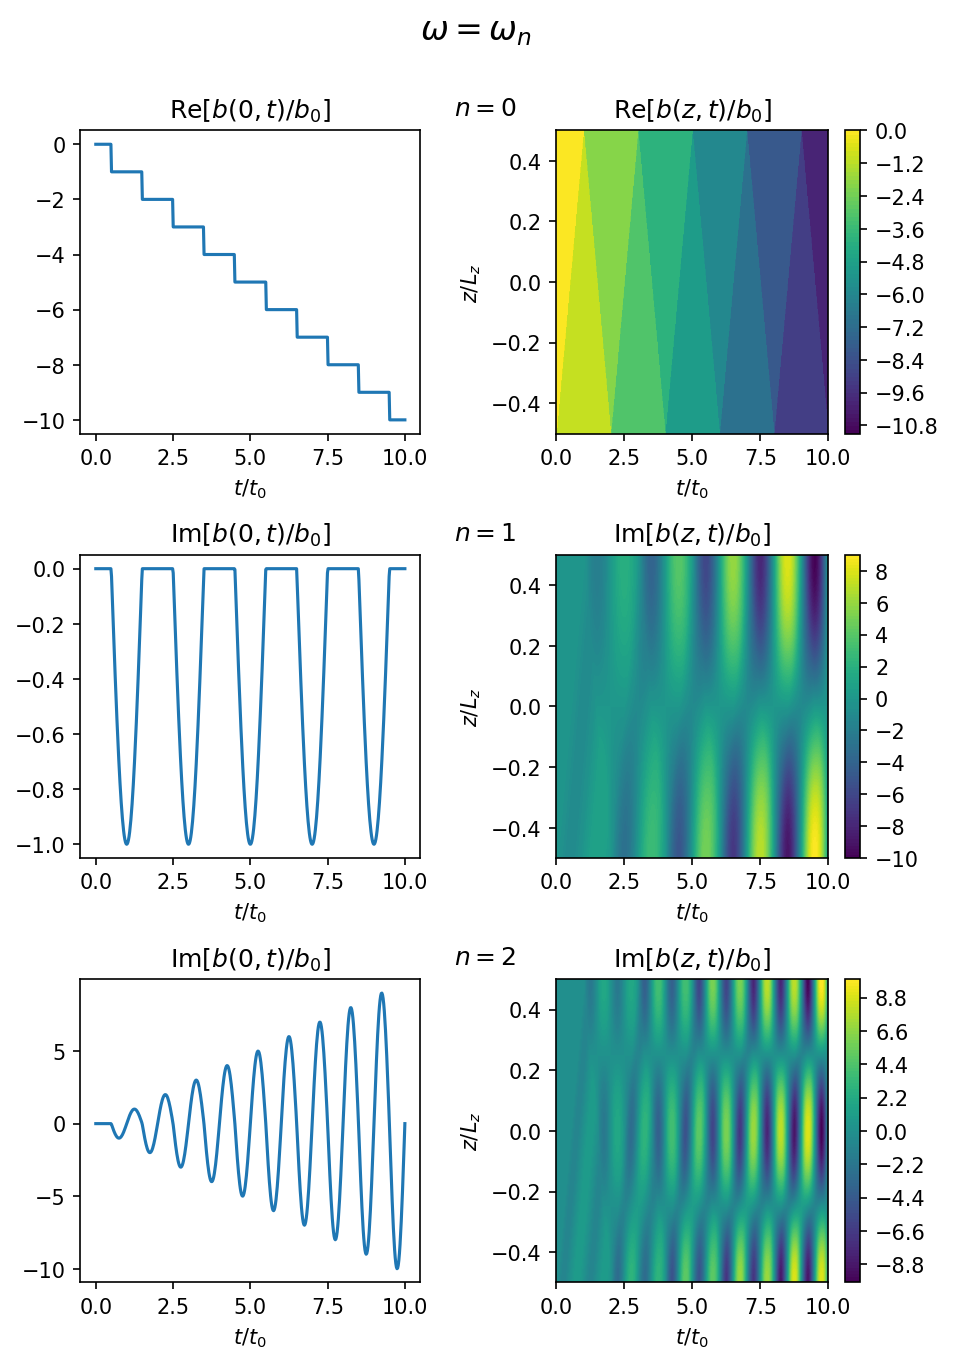
\includegraphics[width=\textwidth,height=0.9\textheight,keepaspectratio]{figures/chapter02/case_where_omega=omega_n_b.png}
    \vspace{-10pt}
    \caption{This figure is very similar to Figure \ref{fig:case_where_omega=omega_n_u} except it shows the magnetic field, $b$, instead of the velocity. The normalising constant, $b_0$, is given by Equation \eqref{eq:b0}. The code used to make this figure is available on GitHub in the following directory:\newline
     \href{https://github.com/aleksyprok/apkp_thesis/blob/main/Python/Chapter2/case_where_omega\%3Domega_n.py}{$\rightarrow$ Python/Chapter2/case\_where\_omega=omega\_n.py}}
    \vspace{-30pt}
    \label{fig:case_where_omega=omega_n_b}
\end{figure}

Figures \ref{fig:case_where_omega=omega_n_u} and \ref{fig:case_where_omega=omega_n_b} show plots of $u$ and $b$ for $\omega=0$, $\omega=\omega_1$ and $\omega_2$. The time is normalised by $t_0$ given by 
\begin{equation}
    \label{eq:t0}
    t_0=\frac{L_z}{v_{A0}}.
\end{equation}
The magnetic field is normalised by $b_0$, given by
\begin{equation}
    \label{eq:b0}
    b_0=\frac{B_0u_0}{v_{A0}.}
\end{equation}
Note that the real component is plotted for $\omega=0$ because the imaginary component gives the trivial solution. The imaginary part is plotted for $n\ge1$ because this ensures $u$ and $b$ are continuous. However, their derivatives are not continuous. In all three plots, the amplitude grows linearly with time, which means the energy grows quadratically. For $n\ge1$, driver generates standing Alfv\'en waves. The time and space averaged kinetic and magnetic energies are approximately equal. For $n=0$, the driver shears the magnetic field, and the amplitude grows linearly with time, whereas the kinetic energy oscillates about a finite value. It is convenient to categorise oscillatory motions into fast and slow motions: Slow motions are where the frequency, $f$, is smaller than $v_{A0}/L_z$, where $L_z$ gives the length of the loop. Fast motions are where the frequency is greater than $v_{A0}/L_z$. A key difference between fast and slow motions is that slow motions can generate a large build-up in magnetic energy with relatively little kinetic energy. For fast motions, the build-up in magnetic energy is approximately equal to the build-up in kinetic energy. The plots show if $u$ has an antinode at a given point in space, then $b$ has a node and vice versa.

\subsection{Approximately resonant case}
\label{sec:case_where_omega_approx_omega_n}

In this section, we investigate the solutions for the case where $\omega = \omega_n + \epsilon \omega_1$, where $\epsilon\ll1$, i.e. we look at the solution where the driving frequency is nearly equal to one of the resonant frequencies.

\begin{figure}
    \centering
    \vspace{-20pt}
    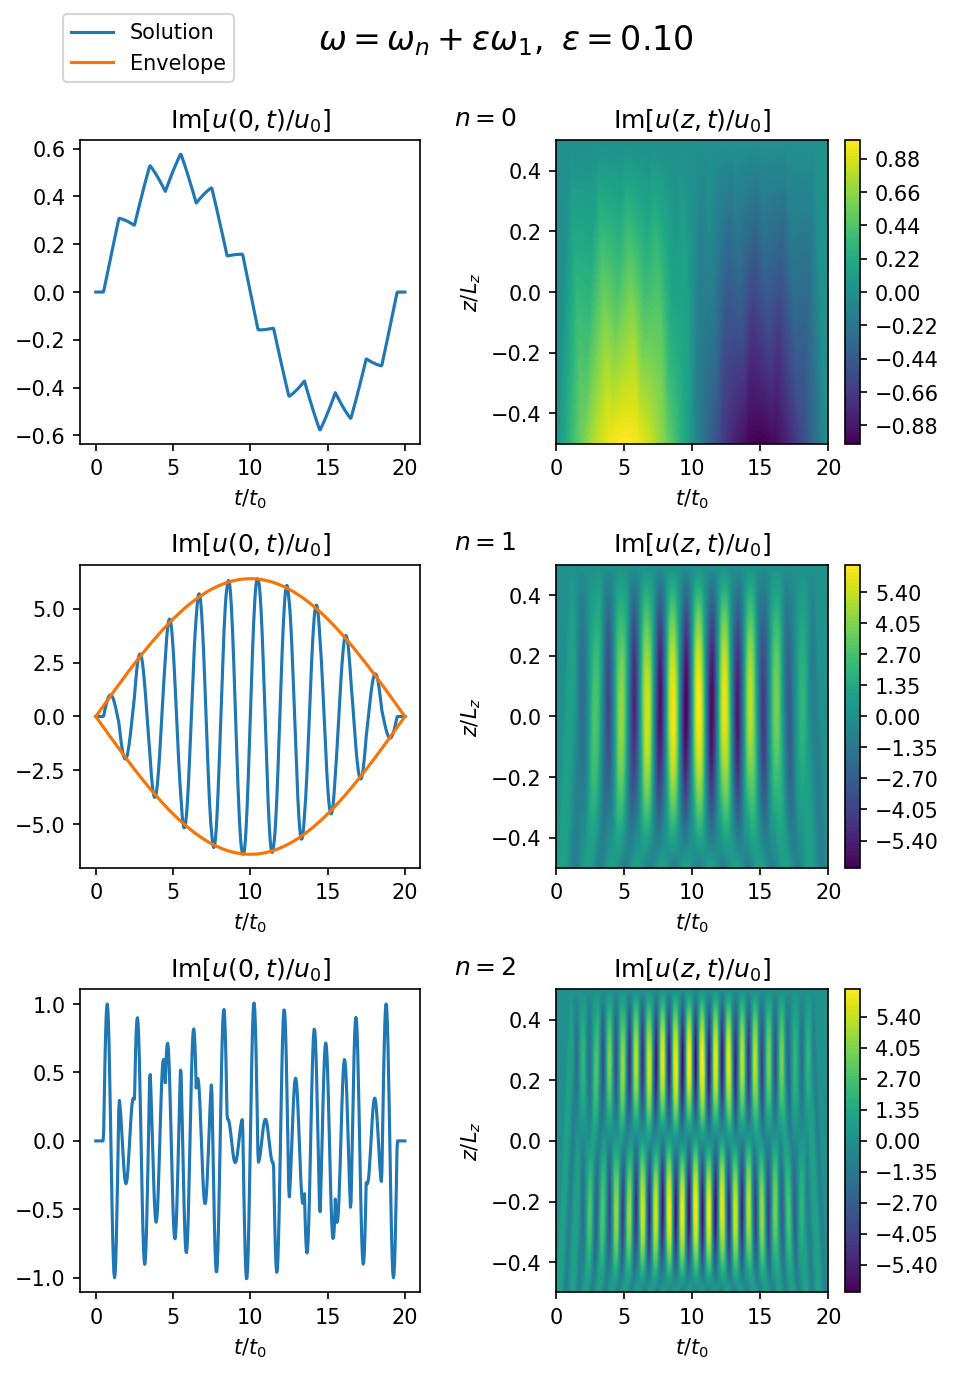
\includegraphics[width=\textwidth,height=0.85\textheight,keepaspectratio]{figures/chapter02/case_where_omega_approx_omega_n_u.png}
    \vspace{-10pt}
    \caption{This figure is similar to Figure \ref{fig:case_where_omega=omega_n_u} except now the frequency is given by $\omega=\omega_n+\epsilon \omega_1$ for $\epsilon=0.1$. Also, the imaginary component is taken for all values of $n$. Note that the velocity at $z=0$ is plotted in blue and the envelope, given by Equation \eqref{eq:u0_envelope}, is plotted in orange. The code used to make this figure is available on GitHub in the following directory:\newline
    \href{https://github.com/aleksyprok/apkp_thesis/blob/main/Python/Chapter2/case_where_omega_approx_omega_n.py}{$\rightarrow$ Python/Chapter2/case\_where\_omega\_approx\_omega\_n.py}}
    \label{fig:case_where_omega_approx_omega_n_u}
    \vspace{-30pt}
\end{figure}

\begin{figure}
    \centering
    \vspace{-20pt}
    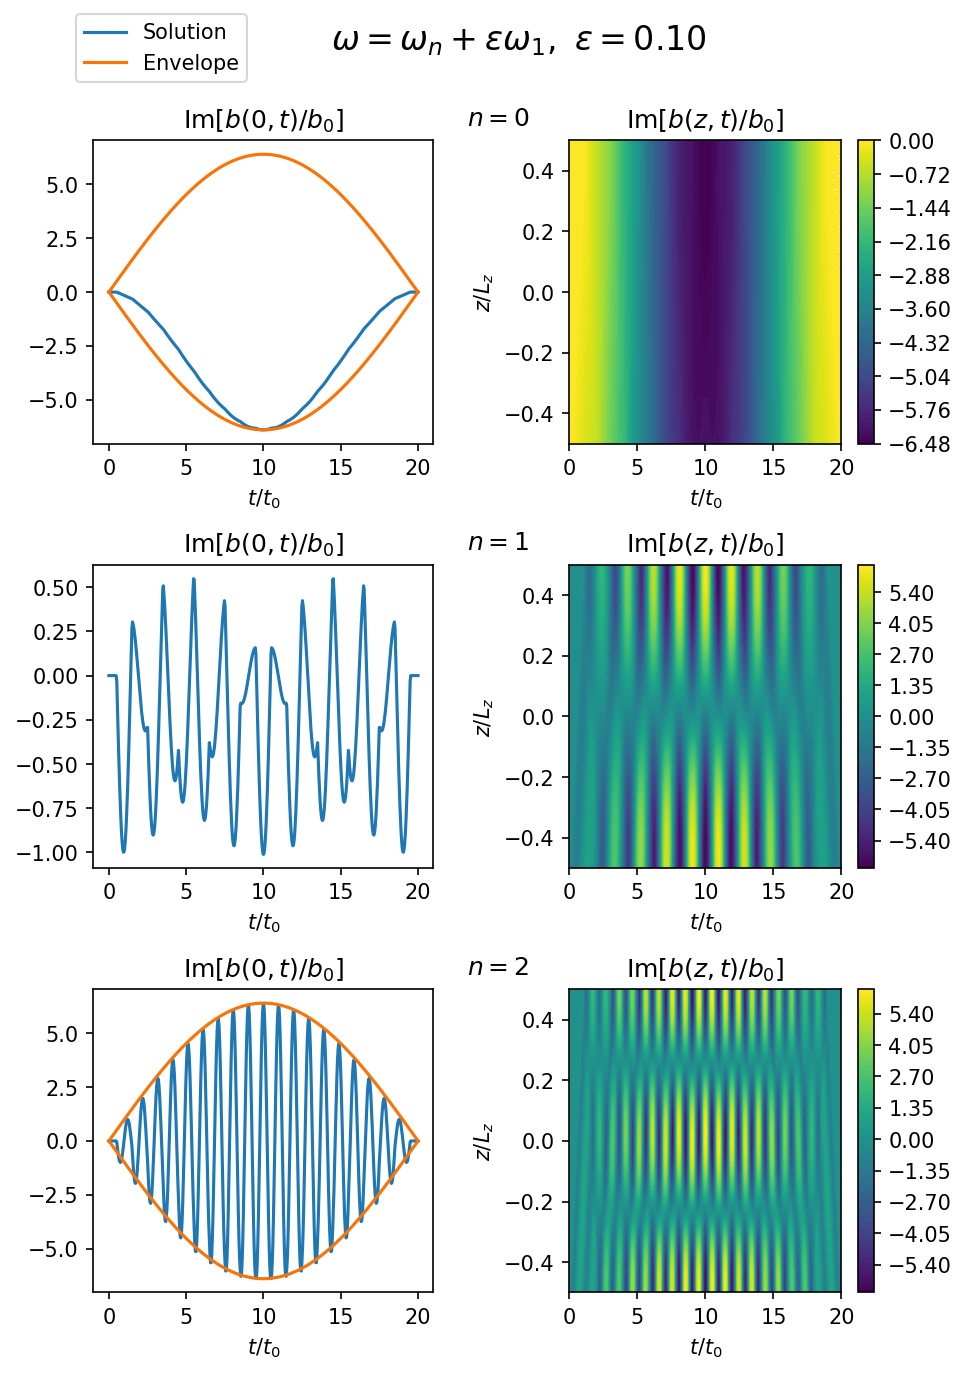
\includegraphics[width=\textwidth,height=0.9\textheight,keepaspectratio]{figures/chapter02/case_where_omega_approx_omega_n_b.png}
    \vspace{-10pt}
    \caption{This figure is similar to Figure \ref{fig:case_where_omega_approx_omega_n_u} except the magnetic field is plotted instead of the velocity. The equation for the envelope is given by Equation \eqref{eq:b0_envelope}. The code used to make this figure is available on GitHub in the following directory:\newline
    \href{https://github.com/aleksyprok/apkp_thesis/blob/main/Python/Chapter2/case_where_omega_approx_omega_n.py}{$\rightarrow$ Python/Chapter2/case\_where\_omega\_approx\_omega\_n.py}}
    \vspace{-30pt}
    \label{fig:case_where_omega_approx_omega_n_b}
\end{figure}

From Equation \eqref{eq:abs_u0_non_res} we know that the absolute value of the velocity at $z=0$ is given by
\[
    |u(0,t)|=u_0\abs{\sec(\frac{\omega l_z}{v_{A0}})\sin\qty{(m'+1)\qty(\frac{l_z}{v_{A0}}(\omega-\omega_n)+\frac{l_z \omega_n}{v_{A0}}+\frac{\pi}{2})}}.
\]
Since $m'+1\in\mathds{Z}$, then for $n$ odd we know that
\[\abs{\sin\qty{(m'+1)\qty(x + \frac{\omega_n l_z}{v_{A0}}+\frac{\pi}{2})}}=\abs{\sin\{(m'+1)x\}}.\]
Therefore, approximating $m'+1$ with 
\[m'+1\approx \frac{v_{A0} t}{L_z},\]
we can derive an equation for an envelope, $u_{e0}(t)$, that that the real and imaginary components of the velocity at $z=0$ approximately lies inside
\begin{equation}
    \label{eq:u0_envelope}
    u_{e0}(t) = \pm u_0\sec\qty(\frac{\omega l_z}{v_{A0}})\sin\qty{\frac{\omega - \omega_n}{2}t},
\end{equation}
for $n$ odd.
Using Equation \eqref{eq:abs_b0_non_res} we can derive a similar envelope, $b_{e0}(t)$ for the magnetic field at $z=0$, given by
\begin{equation}
    \label{eq:b0_envelope}
    b_{e0}(t)=\pm \frac{u_0B_0}{v_{A0}}\csc\qty(\frac{\omega l_z}{v_{A0}})\sin\qty{\frac{\omega - \omega_n}{2}t},
\end{equation}
for $n$ even.

Figures \ref{fig:case_where_omega_approx_omega_n_u} and \ref{fig:case_where_omega_approx_omega_n_b} plot the solutions for the case where $\omega=\omega_n+\epsilon \omega_1$. In all the plots the imaginary part is shown instead of the real part because it is continuous. The plots display an interference pattern called a beat. The beating angular frequency, $\omega_b$, is given by
\begin{equation}
    \omega_b = \frac{\omega - \omega_n}{2}.
\end{equation}
The beat is a concept from acoustics. It is an interference pattern between two sounds of slightly different frequencies, perceived as a periodic variation in magnitude with a rate which is the difference of the two frequencies.

\subsection{Nonresonant case}
\label{sec:case_where_omega_ne_omega_n}

In this section we consider the least resonant case, i.e. the case where
\[\omega = \frac{\omega_{n}+\omega_{n+1}}{2}.\]
This represents the least resonant case because the frequency is as far away from any of the resonant frequencies as possible. The solutions are plotted in Figure \ref{fig:case_where_omega_ne_omega_n_u} and \ref{fig:case_where_omega_ne_omega_n_b}. As expected, maximum energy of the solution is significantly smaller than the maximum energies reached in Figures \ref{fig:case_where_omega=omega_n_u}-\ref{fig:case_where_omega_approx_omega_n_b}. This is because the driver frequency is far away from the resonant and so constructive interference is quickly followed up by destructive interference which prevents the build-up of energy. For $n=3$ and $n=6$ the waves oscillate at a fixed amplitude, then after a time interval of length, $L_z / v_{A0}$, the waves oscillate at a different amplitude.

\begin{figure}
    \centering
    \vspace{-20pt}
    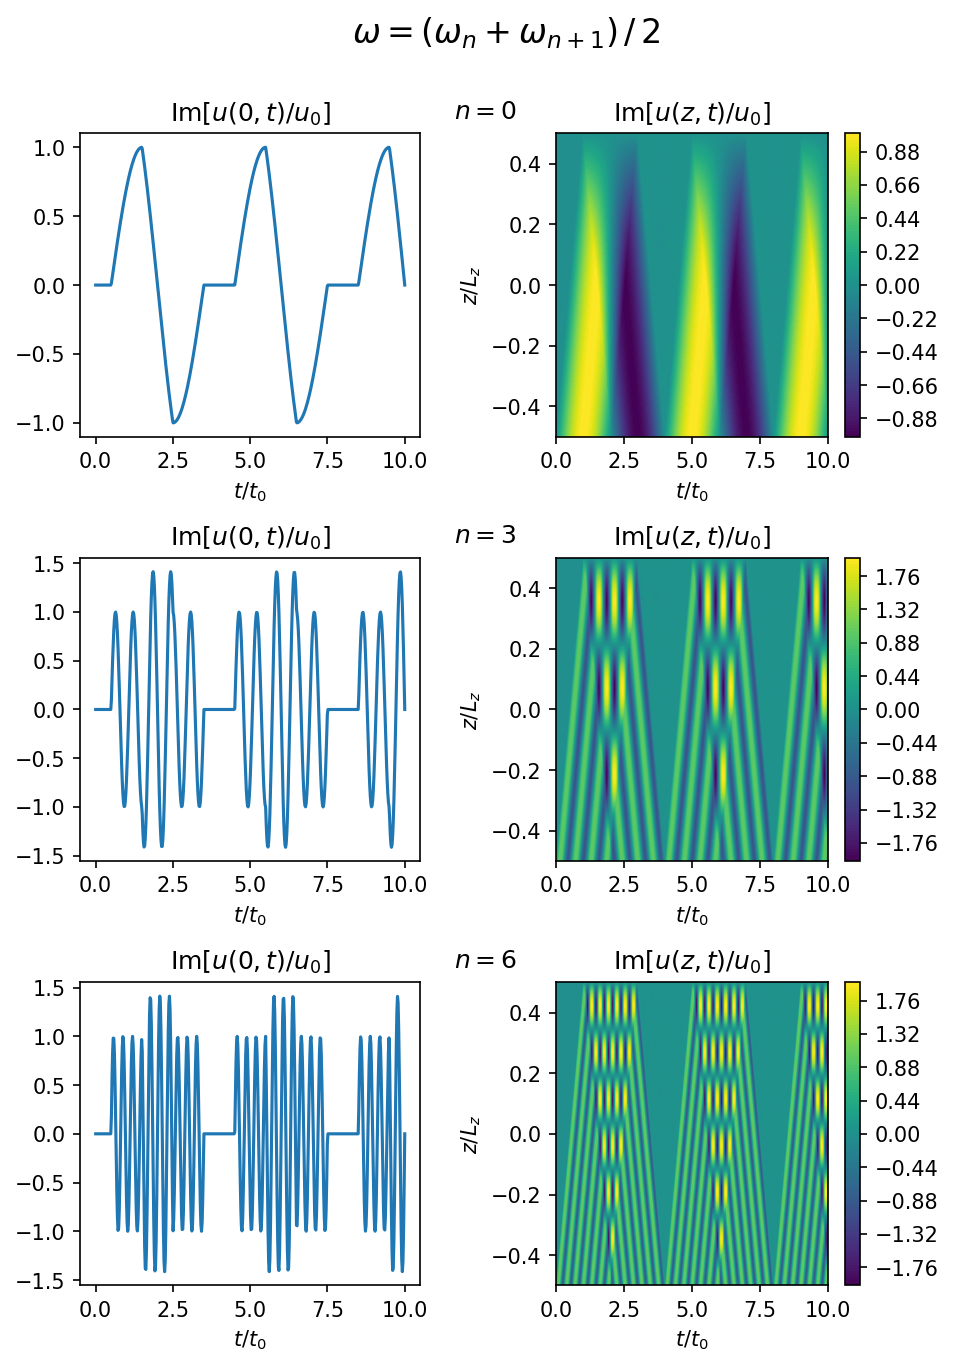
\includegraphics[width=\textwidth,height=0.9\textheight,keepaspectratio]{figures/chapter02/case_where_omega_ne_omega_n_u.png}
    \vspace{-10pt}
    \caption{This figure is similar to Figure \ref{fig:case_where_omega=omega_n_u} except now the frequency is given by $\omega=(\omega_n+\omega_{n+1})/2$. These are the least resonant frequencies because they are as far away from any of the resonant frequencies as possible. The code used to make this figure is available on GitHub in the following directory:\newline
    \href{https://github.com/aleksyprok/apkp_thesis/blob/main/Python/Chapter2/case_where_omega_ne_omega_n.py}{$\rightarrow$ Python/Chapter2/case\_where\_omega\_ne\_omega\_n.py}}
    \vspace{-30pt}
    \label{fig:case_where_omega_ne_omega_n_u}
\end{figure}

\begin{figure}
    \centering
    \vspace{-20pt}
    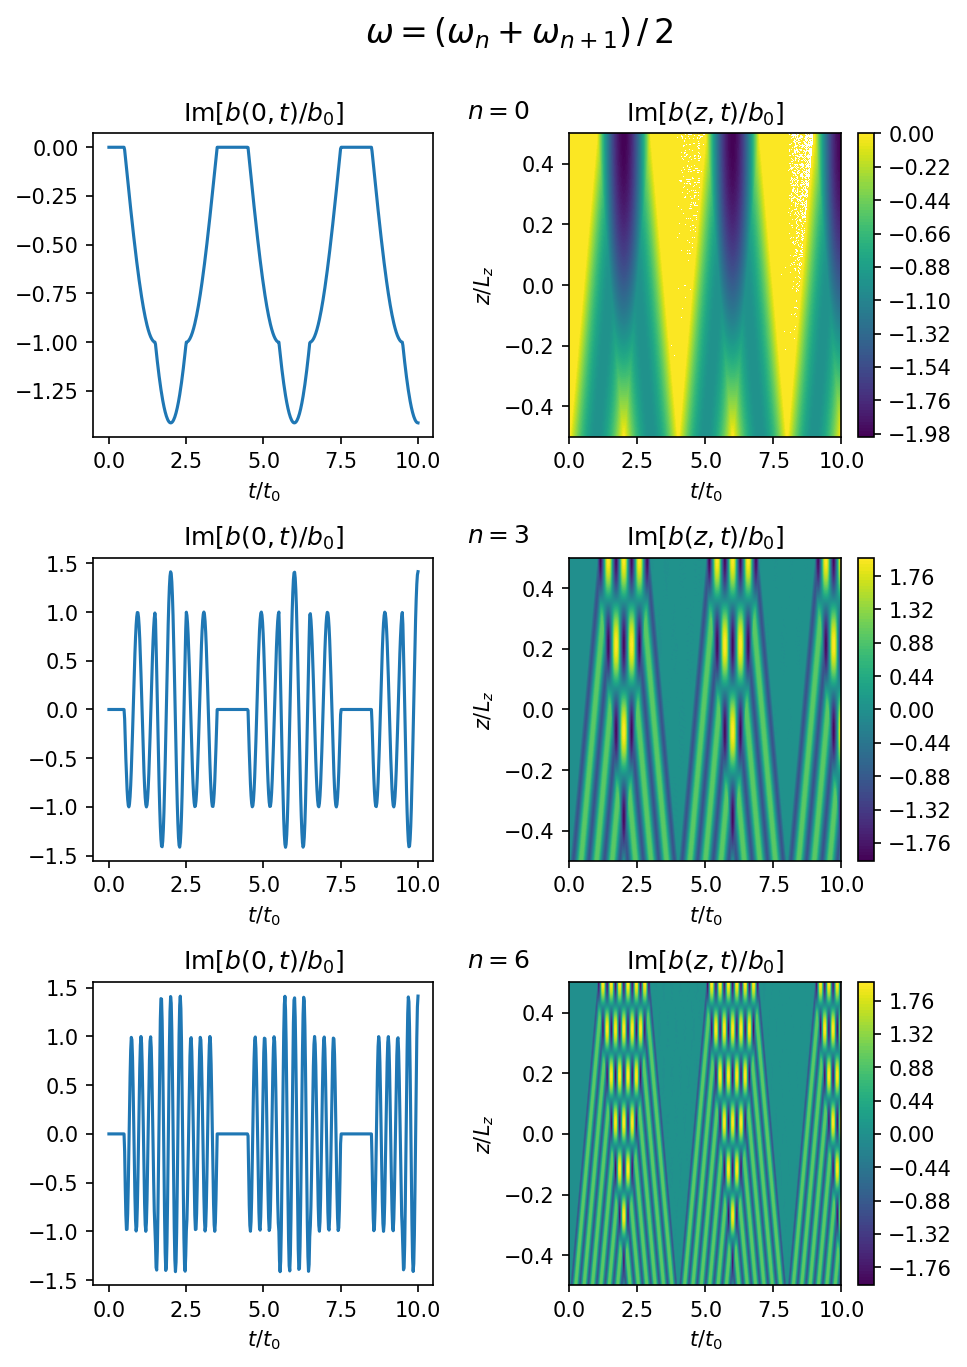
\includegraphics[width=\textwidth,height=0.9\textheight,keepaspectratio]{figures/chapter02/case_where_omega_ne_omega_n_b.png}
    \vspace{-10pt}
    \caption{This figure is similar to Figure \ref{fig:case_where_omega=omega_n_u} except the magnetic field is plotted instead of the velocity. The code used to make this figure is available on GitHub in the following directory:\newline
    \href{https://github.com/aleksyprok/apkp_thesis/blob/main/Python/Chapter2/case_where_omega_ne_omega_n.py}{$\rightarrow$ Python/Chapter2/case\_where\_omega\_ne\_omega\_n.py}}
    \vspace{-30pt}
    \label{fig:case_where_omega_ne_omega_n_b}
\end{figure}

\section{Closed loop: broadband driver}
\label{sec:closed_loop_random_driver}

This section takes a statistical approach to study the solutions for a broadband driver, i.e. a driver which excites a wide range of frequencies. The previous section calculated the solution for a single frequency driver. Figure \ref{fig:power_spectrum_morton} shows that velocity fluctuations in the corona oscillate at a wide range of frequencies. We think of the previous section as the case where the driver includes only one term in its Fourier series. In contrast, this section contains many terms, even an infinite number of terms. We can constrain the terms' amplitude using observed power spectra, e.g. Figure \ref{fig:power_spectrum_morton}. However, each term's phase cannot be constrained. Therefore, we need to consider all possible phases associated with each term in the Fourier series. Given the infinite number of possibilities, we take a statistical approach to study the solutions. We aim to study the average behaviour and answer the question: do the solutions grow to infinity or oscillate about a finite value? In the previous section, we calculated that for a sinusoidal driver, the solution's energy either oscillates about a finite value if $\omega\ne\omega_n$ or grows to infinity if $\omega=\omega_n$. To answer this question for the broadband driver, we first reduce Equation \eqref{eq:alfven_wave_equation2} to a system of ODEs, corresponding to the equation of a driven harmonic oscillator. After that, we calculate the general solution to the ODE, and then we study the case where the driver gives a red noise and white noise force.

\subsection{Driven harmonic oscillator}
\label{sec:chap_2_driven_harmonic_oscillator}

We define our $z$-range to be given by $0\le z\le L_z$ with the boundary conditions given by
\begin{equation}
    u(0,t) = f_{driv}(t),\quad u(L_z,t) = 0.
\end{equation}
Let
\begin{equation}
    u(z,t) = y(z,t) + \frac{L_z - z}{L_z}f_{driv}(t).
\end{equation}
Substituting this into Equation \eqref{eq:alfven_wave_equation2} gives
\begin{equation}
    \begin{aligned}
    \pdv[2]{y}{t}-v_{A0}^2\pdv[2]{y}{z}&=-\frac{L_z - z}{L_z}\dv[2]{f_{driv}}{t} \\
    \end{aligned}
\end{equation}
Hence, the boundary conditions for $y(z,t)$ are
\begin{equation}
    y(\pm l_z, t) = 0.
\end{equation}
We can equate the right-hand side with the following Fourier series
\begin{equation}
    -\frac{L_z - z}{L_z}f_{driv}''(t) = -2f_{driv}''(t)\sum_{n=1}^\infty \frac{\sin(k_{zn} z)}{n\pi},
\end{equation}
for $0<z\le L_z$, where
\begin{equation}
    k_{zn} = \frac{n\pi}{L_z}.
\end{equation}
Let
\begin{equation}
    y(z,t) = \sum_{n=1}^\infty y_n(t)\sin(k_{zn}z),
\end{equation}
therefore, each $y_n$ satisfies
\begin{equation}
    \label{eq:driven_harmonic_oscillator}
    \dv[2]{y_n}{t} + \omega_n^2y_n=f_n(t),
\end{equation}
where 
\begin{gather}
    \omega_n = \frac{n\pi}{L_z}v_{A0},
    f_n(t) = -2\frac{f_{driv}''(t)}{n\pi}.
\end{gather}
Note that Equation \eqref{eq:driven_harmonic_oscillator} is the equation for a driven harmonic oscillator.

\subsection{General solution}

In this section we calculate the general solution to Equation \eqref{eq:driven_harmonic_oscillator}. We first calculate a general solution using a Green's function. After that, we calculate the mean and variance of the solution for a driver with a Fourier series where each coefficient is a random number from a Gaussian probability distribution.

The Green's function, $G(t)$ for Equation \eqref{eq:driven_harmonic_oscillator} is
\begin{equation}
    G(t) = H(t)\frac{\sin(\omega_n t)}{\omega_n},
\end{equation}
where $H(t)$ is the Heaviside step function.
We impose the initial condition
\begin{equation}
    \label{eq:initial_conditions_greens_function}
    y_n(0)=\left.\dv{y_n}{t}\right|_{t=0}=0,
\end{equation}
therefore, the complementary component of the solution is zero. Hence, the general solution is given by
\begin{equation}
    \label{eq:general_soln_greens_function}
    y_n=\frac{1}{\omega_n}\int_0^t\sin[\omega_n(t-t')]f_n(t')dt'.
\end{equation}

Equation \eqref{eq:general_soln_greens_function} works for any smooth function. Now we will consider the solution where we know the Fourier series of the driver up to a statistical average. Let the following Fourier series describe $f_n(t)$,
\begin{equation}
    \label{eq:random_fourier_series}
    f_n(t)=a_0X_0 + \sum_{k=1}^\infty a_k X_k\cos(\omega_kt) + b_k Y_k \sin(\omega_k t),
\end{equation}
for $t\in[0,P]$, where
\begin{equation}
    \label{eq:omega_k}
    \omega_k = \frac{k \pi}{2P},
\end{equation}
$X_k$, $Y_k$ are independent random Gaussian variables with mean, 
\[\langle X_k \rangle = \langle Y_k \rangle = 0,\]
and variance
\[\langle X_k^2 \rangle = \langle Y_k^2 \rangle = 1.\]
Therefore, by Parseval's theorem,
\begin{equation}
    \frac{1}{2P}\int_0^{2P}f_n^2(t)dt = a_0^2X_0^2+\frac{1}{2}\sum_{k=1}^\infty a_k^2X_k^2 + b_k^2Y_k^2.
\end{equation}
Hence,
\begin{equation}
\begin{aligned}
   \left\langle\frac{1}{2P}\int_0^{2P}f_n^2(t)dt\right\rangle &= \langle a_0^2X_0^2 \rangle +\frac{1}{2}\sum_{k=1}^\infty \langle a_k^2X_k^2 \rangle + \langle b_k^2Y_k^2 \rangle \\
    &= a_0^2+\frac{1}{2}\sum_{k=1}^\infty a_k^2 + b_k^2.
\end{aligned}
\end{equation}
Therefore, the coefficients $a_k$, $b_k$ give the average power spectrum of $f_n(t)$. We can use data from observations, e.g. Figure \ref{fig:power_spectrum_morton} to determine the values of $a_k$, $b_k$.

Using Equation \eqref{eq:general_soln_greens_function}, the solution for $f_n(t)$ given by Equation \eqref{eq:random_fourier_series} is
\begin{equation}
    \label{eq:velocity_soln_random_fourier_driver}
    y_n(t) = \sum_{k=0}^\infty y_n^{(k)}(t),
\end{equation}
where
\begin{equation}
    y_n^{(k)}(t) = \frac{a_k X_k\omega_n\qty[\cos(\omega_n t) - \cos(\omega_k t)] + b_k Y_k\qty[\omega_k\sin(\omega_n t) - \omega_n\sin(\omega_k t)]}{\omega_n(\omega_k^2 - \omega_n^2)},
\end{equation}
for $\omega_k\ne \omega_n$ and
\begin{equation}
    y_n^{(k)}(t) = \frac{a_k X_k\omega_n t \sin(\omega_n t) + b_k Y_k\qty[\sin(\omega_n t) - \omega_n t \cos(\omega_n t)]}{2\omega_n^2},
\end{equation}
for $\omega_k = \omega_n$. Therefore, the mean $\langle y_n(t) \rangle = 0$ and the variance is given by
\begin{equation}
    \label{eq:variance_fourier}
    \langle y_n^2(t) \rangle = \sum_{k=0}^\infty \left\langle \qty[y_n^{(k)}(t)]^2 \right\rangle,
\end{equation}
where
\begin{equation}
    \label{eq:variance_omega_ne_omega_k}
    \left\langle \qty[y_n^{(k)}(t)]^2 \right\rangle = \frac{a_k^2 \omega_n^2\qty[\cos(\omega_n t) - \cos(\omega_k t)]^2 + b_k^2 \qty[\omega_k\sin(\omega_n t) - \omega_n\sin(\omega_k t)]^2}{\omega_n^2(\omega_k^2 - \omega_n^2)^2},
\end{equation}
for $\omega_k\ne\omega_n$ and
\begin{equation}
    \label{eq:variance_omege=omega_k}
    \left\langle \qty[y_n^{(k)}(t)]^2 \right\rangle = \frac{a_k^2 \omega_n^2 t^2 \sin^2(\omega_n t) + b_k^2 \qty[\sin(\omega_n t) - \omega_n t \cos(\omega_n t)]^2}{4\omega_n^4},
\end{equation}
if $\omega_k=\omega_n$. This shows that in general, the power spectrum will have a peak at the resonant frequencies.

Here we calculate the time-derivative of the variance because we will need it in Section \ref{sec:noisy_force}. The time-derivative of $y_n(t)$ is given by
\begin{equation}
    \dv{y_n}{t} = \sum_{k=0}^\infty\dv{y_n^{(k)}}{t},
\end{equation}
where
\begin{equation}
    \dv{y_n^{(k)}}{t} = \frac{a_k X_k\qty[\omega_k\sin(\omega_k t) - \omega_n\sin(\omega_n t) ] + b_k Y_k \omega_k\qty[\cos(\omega_n t) - \cos(\omega_k t)]}{\omega_k^2 - \omega_n^2},
\end{equation}
for $\omega_k\ne \omega_n$ and
\begin{equation}
    \label{eq:variance_d_velocity_dt}
    \dv{y_n^{(k)}}{t} = \frac{a_k X_k [\sin(\omega_n t) + \omega_n t \cos(\omega_n t)]+ b_k Y_k \omega_n t \sin(\omega_n t)}{2\omega_n},
\end{equation}
for $\omega_k = \omega_n$. Therefore, the mean $\langle \dv*{y_n}{t} \rangle = 0$ and the variance is given by
\begin{equation}
    \left\langle \qty[\dv{y_n}{t}]^2 \right\rangle = \sum_{k=0}^\infty \left\langle \qty[\dv{y_n^{(k)}}{t}]^2 \right\rangle,
\end{equation}
where
\begin{equation}
    \left\langle \qty[\dv{y_n^{(k)}}{t}]^2 \right\rangle = \frac{a_k^2\qty[\omega_k\sin(\omega_k t) - \omega_n\sin(\omega_n t)]^2 + b_k^2\omega_k^2 \qty[\cos(\omega_n t) - \cos(\omega_k t)]^2}{(\omega_k^2 - \omega_n^2)^2},
\end{equation}
for $\omega_k\ne\omega_n$ and
\begin{equation}
   \left\langle \qty[\dv{y_n^{(k)}}{t}]^2 \right\rangle = \frac{a_k^2 [\sin(\omega_n t) + \omega_n t \cos(\omega_n t)]^2+ b_k^2  \omega_n^2 t^2 \sin^2(\omega_n t)}{4\omega_n^2},
\end{equation}
if $\omega_k=\omega_n$.

\subsection{Noisy force}
\label{sec:noisy_force}

Let $\eta(t)$ be a noisy signal, given by
\begin{equation}
    \eta(t) = \int_{-\infty}^\infty \hat{\eta}(f)\exp(2\pi i t f) df,
\end{equation}
where its Fourier transform in the sense of distributions, $\hat{\eta}(f)$, is given by
\begin{equation}
    \begin{aligned}
    \hat{\eta}(f) &= \int_{-\infty}^\infty \eta(t)\exp(-2\pi i t f) dt, \\
    \end{aligned}
\end{equation}
where $f$ denotes the frequency. We define $\eta(t)$ to be a white noise signal of strength $D$. The value of $\eta(t)$ for any time $t$ is a random Gaussian variable that is statistically independent of its entire history before. Its power spectrum is given by
\begin{equation}
    \left\langle|\hat{\eta}(f)|^2\right\rangle = D,
\end{equation}
where $D$ is a constant.
Similarly, we define $W(t)$ to be red noise of strength $E$ if it is a random signal with a power spectrum given by
\begin{equation}
    \left\langle|\hat{W}(f)|^2\right\rangle = E f^{-2},
\end{equation}
where $E$ is a constant. Red noise is often called brown noise due to its association with Brownian motion. We think of it as the integral of white noise, and it is closely related to the Wiener process. The colour of the noise takes its name from its power spectrum. White noise excites all frequencies equally and is analogous to visible white light which contains all frequencies in the rainbow. Red noise has more energy in the lower frequencies, similar to visible red light and is at the lower end of the visible light frequency spectrum.

Let the displacement, $x_n$, be given by
\begin{equation}
    \dv{x_n}{t} = y_n.
\end{equation}
Let the acceleration, $g_n$, be given by
\begin{equation}
    \dv{g_n}{t} = f_n.
\end{equation}
Substituting the above two equations into Equation \eqref{eq:driven_harmonic_oscillator} and integrating gives
\begin{equation}
    \label{eq:driven_harmonic_oscillator_displacement}
    \dv[2]{x_n}{t} + \omega_n^2x_n=g_n(t) + C,
\end{equation}
where $C$ is an integration constant. We consider the case where the integration constant $C$ equals 0 as the solution associated with this term can be superimposed if needed. Equation \eqref{eq:driven_harmonic_oscillator_displacement} shows that $g_n(t)$ has the dimensions of a force (divided by mass). Therefore, if $g_n(t)=\eta(t)$ we say the system is driven by a white noise force and if $g_n(t)=W(t)$ then the system is driven by a red noise force. We are interested in red and white noise because they power produce spectra with slopes $f^0$ and $f^{-2}$. Fitting Figure \ref{fig:power_spectrum_morton} with a single power law shows the velocity fluctuations in the solar corona have a power spectrum which goes as $f^p$, where $-2<p<0$. If $g_n(t)=\eta(t)$, then we solve Equation \eqref{eq:driven_harmonic_oscillator_displacement}. If $g_n(t)=W(t)$, then $f_n(t)=\eta(t)$ and so we solve Equation \eqref{eq:driven_harmonic_oscillator}. In other words, we solve the equation where white noise is on the right hand side. In this section we will solve for the case where $g_n(t)=W(t)$, then we use a trick where we substitute $\dv*{y_n}{t}\rightarrow y_n$ to quickly calculate the solution for the case where $g_n = \eta(t)$. Note that this substitution causes the initial conditions, see Equation \eqref{eq:initial_conditions_greens_function}, to change to 
\begin{equation}
    x_n(0) = \dv{x_n}{t} = 0.
\end{equation}

By the Wiener–Khinchin theorem, $\eta(t)$ has an autocorrelation given by the Fourier transform of the power spectral density, i.e.
\begin{equation}
    \label{eq:autocorrelation}
    \begin{aligned}
    \langle\eta(t) \eta(t')\rangle &= \int_{\infty}^\infty \left\langle\abs{\hat{\eta}(\xi)}^2\right\rangle\exp[2\pi i \xi (t - t')] d\xi \\
    &=D\delta(t-t'),
    \end{aligned}
\end{equation}
where $\delta(t-t')$ is the Dirac delta function. 
If $f_n(t)$ is a white noise signal then Equation \eqref{eq:driven_harmonic_oscillator} gives a Langevin equation where an exact solution can be calculated with a simpler solution compared with Equation \eqref{eq:driven_harmonic_oscillator}. Substituting $f_n(t)=\eta(t)$ into Equation \eqref{eq:driven_harmonic_oscillator} gives the following Langevin equation
\begin{equation}
    \dv[2]{y_n}{t} + \omega_n^2 y_n = \eta(t).
\end{equation}
Note that $\eta(t)$ has a mean of
\begin{equation}
    \langle\eta(t)\rangle=0.
\end{equation}
Using Equation \eqref{eq:general_soln_greens_function}, the solution is given by
\begin{equation}
    y_n = \frac{1}{\omega_n}\int_0^t\sin[\omega_n(t-t')]\eta(t')dt',
\end{equation}
and
\begin{equation}
    \dv{y_n}{t} = \int_0^t\cos[\omega_n(t-t')]\eta(t')dt'.
\end{equation}
Hence, the mean of $y_n$ is given by
\begin{equation}
    \begin{aligned}
    \langle y_n \rangle &= \frac{1}{\omega_n}\int_0^t\sin[\omega_n(t-t')]\langle \eta(t') \rangle dt' \\
    &= 0.
    \end{aligned}
\end{equation}
The square of $y_n$ is given by
\begin{equation}
    y_n^2 = \frac{D^2}{\omega_n^2}\int_0^t\int_0^t\sin[\omega_n(t-t')]\sin[\omega_n(t-t'')]\eta(t')\eta(t'')dt'dt''.
\end{equation}
Hence, the variance of $y_n$ is given by
\begin{equation}
    \label{eq:variance_exact_red_force}
    \begin{aligned}
    \langle y_n^2 \rangle &= \frac{1}{\omega_n^2}\int_0^t\int_0^t\sin[\omega_n(t-t')]\sin[\omega_n(t-t'')]\langle \eta(t')\eta(t'')\rangle dt'dt'' \\
    &= \frac{D}{\omega_n^2}\int_0^t\int_0^t\sin[\omega_n(t-t')]\sin[\omega_n(t-t'')]\delta(t'-t'') dt'dt'' \\
    &= \frac{D}{\omega_n^2}\int_0^t\sin^2[\omega_n(t-t')] dt' \\
    &=\frac{D}{2\omega_n^3}[\omega_n t - \sin(\omega_n t) \cos(\omega_n t)].
    \end{aligned}
\end{equation}
Similarly, the mean of $\dv*{y_n}{t}$ is 
\begin{equation}
    \left\langle \dv{y_n}{t} \right\rangle=0.
\end{equation}
The variance is given by
\begin{equation}
    \left\langle \qty[\dv{y_n}{t}]^2 \right\rangle=\frac{D}{2\omega_n}[\omega_n t + \sin(\omega_n t) \cos(\omega_n t)].
\end{equation}
This shows that for both a red/white noise driver the energy on average goes to infinity. For a single frequency resonant driver the amplitude grows linearly with time whereas for a white/red noise driver, the standard deviation grows as $\sqrt{t}$. However, white noise drivers are unphysical because they have an infinite variance. The variance of $\eta(t)$ is given by its autocorrelation for $t=t'$. Equation \eqref{eq:autocorrelation} shows that variance is infinite, and this is because white noise excites all the frequencies from $0$ to $\infty$. Equation \eqref{eq:variance_omega_ne_omega_k} shows that the variance associated with the higher frequency drivers goes to $0$ as $f\rightarrow\infty$. For this reason, we predict the solutions above provide a good approximation for solutions where the driver only excites frequencies up to a finite value, provided the resonant frequency is excited. To test this prediction, the next paragraph calculates the solution for a more physical driver which excites a finite range of frequencies causing it to have a finite variance.

Our goal is to ensure $f_n(t)$ excites each frequency with the same strength as $\eta(t)$ but only for a finite number of frequencies.
Note that Equation \eqref{eq:random_fourier_series} can be written as
\begin{equation}
    f_n(t) = \sum_{k=-\infty}^\infty C_k\exp[2\pi i f_k t] \Delta f,
\end{equation}
where
\begin{gather}
     C_k = \begin{cases}
    4Pa_0 X_0, & k=0, \\
    2P(a_kX_k - i b_k Y_k), & k>0, \\
    C^*_{\abs{k}}, k<0,
    \end{cases} \\
    f_k = \frac{k}{4P}, \\
    \Delta f = \frac{1}{4P}.
\end{gather}
For $P\rightarrow\infty$
\[f_k \rightarrow f,\]
\[\Delta f \rightarrow df,\]
\[C_k \rightarrow C(f),\]
hence,
\begin{equation}
    f_n(t) \rightarrow \int_{-\infty}^\infty C(f) \exp[2\pi i f t] df.
\end{equation}
By the Wiener–Khinchin theorem,
\begin{equation}
    \begin{aligned}
    \implies \langle f_n^2(t)\rangle &= \sum_{k=-\infty}^\infty \left\langle\abs{C_k}^2\right\rangle\exp[2\pi i f t] \\
    &\rightarrow \int_{-\infty}^\infty \left\langle\abs{C(f)}^2\right\rangle \exp[2\pi i f t] d f. \\
    \end{aligned}
\end{equation}
Hence, we require
\begin{equation}
    \left\langle\abs{C_k}^2\right\rangle = \frac{D}{\Delta f}.
\end{equation}
Note that
\begin{equation}
    \langle \abs{C_k}^2 \rangle = \begin{cases}
    (4Pa_0)^2, & k=0, \\
    4P^2(a_k^2 + b_k^2), & k\ne0,
    \end{cases}
\end{equation}
therefore, letting $a_k=b_k$ gives
\begin{equation}
\label{eq:coeffs_ak_bk}
\implies
    \begin{pmatrix}
    a_0 \\
    a_k \\
    b_k
    \end{pmatrix}
    = \frac{1}{2}\sqrt{\frac{D}{P}}
    \begin{pmatrix}
    1 \\
    \sqrt{2} \\
    \sqrt{2}
    \end{pmatrix}.
\end{equation}
Equation \eqref{eq:variance_fourier}, with the coefficients above gives an  $f_n(t)$ which excites each frequency with the same strength as $\eta(t)$ but only for a finite number of frequencies.

\begin{figure}
    \centering
    \vspace{-20pt}
    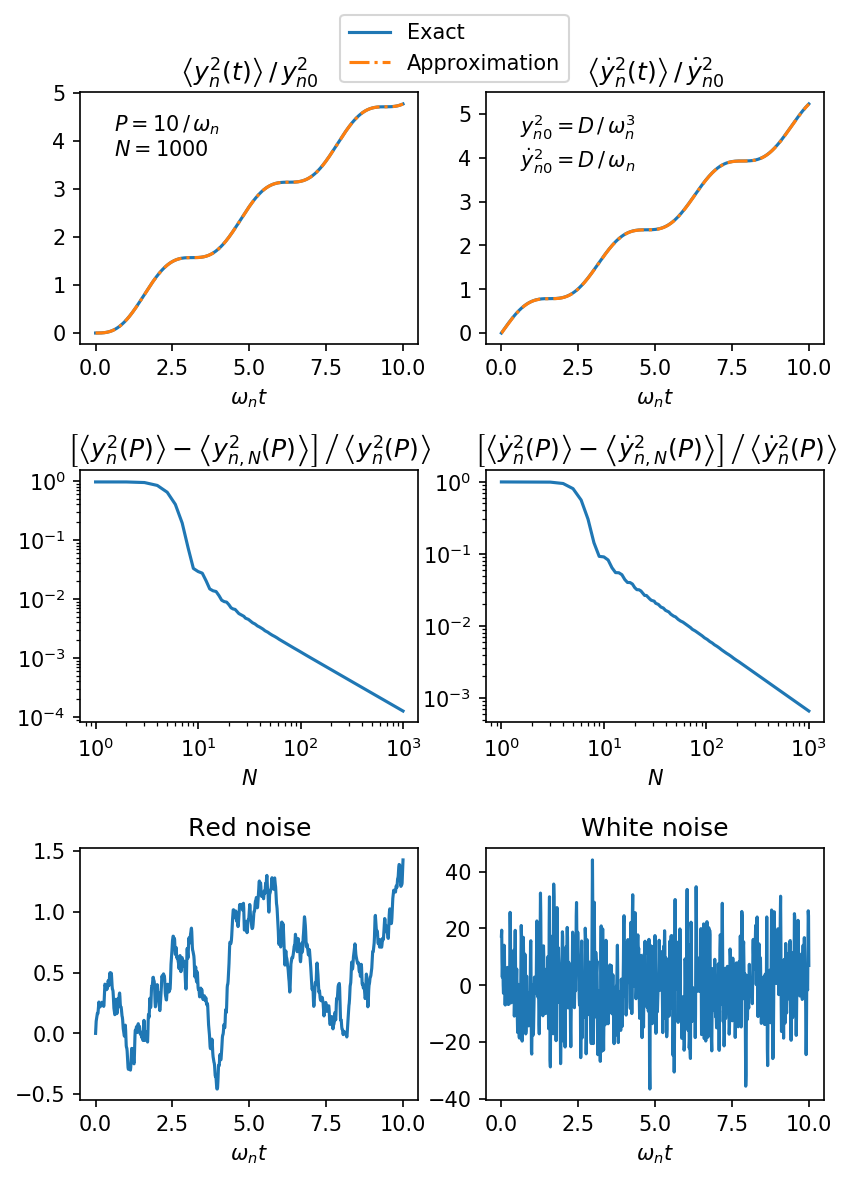
\includegraphics[width=\textwidth,height=0.8\textheight,keepaspectratio]{figures/chapter02/noisy_driver.png}
    \vspace{-10pt}
    \caption{This figure's top row shows the normalised variance of $y_n$ and $\dot{y}_n$, where we use Newton's dot notation to denote the time derivative. They plot the exact solution and the Fourier approximations. The equations for the normalising constants, $y_{n0}$ and $\dot{y}_{n0}$ is also shown. The middle row shows the error at $t=P$ between the exact solution and the Fourier approximation as a function of the number of terms in the approximation. Finally, the bottom row illustrates an example of red and white noise. The code used to make this figure is available on GitHub in the following directory:\newline
    \href{https://github.com/aleksyprok/apkp_thesis/blob/main/Python/Chapter2/random_driver.py}{$\rightarrow$ Python/Chapter2/random\_driver.py}}
    \vspace{-20pt}
    \label{fig:noisy_driver}
\end{figure}

Our goal now is to test our prediction that Equation \eqref{eq:variance_fourier} gives the same solution as Equation \eqref{eq:variance_exact_red_force} with the coefficients given by Equation \eqref{eq:coeffs_ak_bk}. We approximate the sum given by Equation \eqref{eq:variance_fourier} numerically and so the series is truncated at $k=N$. We denote that truncated approximation of Equation \eqref{eq:variance_fourier} with
\begin{equation}
    \label{eq:variance_fourier_truncated}
    \langle y_{n,N}(t) \rangle =\sum_{k=0}^N \langle y_n^{(k)} \rangle.
\end{equation}
We refer to the solution given by Equation \eqref{eq:variance_fourier_truncated} as the Fourier approximation and the solution given by Equation \eqref{eq:variance_exact_red_force} as the exact solution. The top row of Figure \ref{fig:noisy_driver} shows the variance of $y_n$ and its time derivative. It shows that for $P=10/\omega_n$ and $N=1000$ that the exact solution and Fourier approximation are in approximate agreement. The second row shows the error for the variance at $t=P$ between the exact solution and the Fourier approximation as a function of the number of terms in the truncated Fourier series. It shows that increasing the number of terms causes the error to decrease. Note that $P=10/\omega_n$, therefore, from Equation \eqref{eq:omega_k} we know that
\[\omega_k = \frac{k\pi}{20}\omega_n,\]
hence, $\omega_k>\omega_n$ for $k>6$.
The middle row of Figure \ref{fig:noisy_driver} shows that for $N\approx6$, the accuracy sharply improves for increasing $N$. This suggests that provided the resonant frequency is excited then the exact solution and Fourier approximation show approximate agreement. Therefore, the solution given by white noise which only excites frequencies over a finite range can approximate the solution given by $\eta(t)$ which excites all the frequencies from 0 to $\infty$. Finally, the bottom row of Figure \ref{fig:noisy_driver} shows an illustration of red and white noise. The white noise plot was produced using a truncated approximation of Equation \eqref{eq:random_fourier_series}, with $N=1000$. The red noise plots show the time integral of the white noise plot. The white noise plot shows an example of white noise where only a finite range of frequencies is excited. Note that it has a finite variance, whereas, $\eta(t)$, which excites all frequencies, has an infinite variance.

\section{Leaky loop: reflection coefficient}
\label{sec:leaky_loop_reflection_coefficent}

In previous sections, we modelled the boundary of the domain as a solid wall. This is a good leading order approximation for the boundary between the corona and the lower layers of the atmosphere. Figure \ref{fig:VAL_atmosphere} shows that the chromosphere and photosphere are orders of magnitude denser than the corona. We can approximate this as a solid wall, provided the wavelength of the waves is significantly longer than length-scale of the density variations. In this section, we aim to calculate an approximation for the Alfv\'en wave reflection coefficient at the corona/chromosphere interface. In other words, we aim to calculate on average how much energy is reflected and transmitted for waves at the boundary of the corona. In previous sections, we modelled perfect reflection, i.e. we assumed 100\% of the energy reflects at the boundary.  Therefore, we described the loops as closed. In this section, the reflection coefficient is less than unity so that some energy can escape. Therefore, we describe the loops as leaky.

To estimate the reflection coefficient, we use a method very similar to that described in \citet{Hollweg1984b}. We model the background Alfv\'en speed as 
\begin{equation}
    \label{eq:alfven_speed_exponential}
    v_A(z) = \begin{cases}
    v_{A0}\exp(z/(2h)), & z < 0, \\
    v_{A0}, & z\ge 0, \\
    \end{cases}
\end{equation}
where $h$ gives the pressure scale height which is defined as
\begin{equation}
    \label{eq:pressure_scale_height}
    h = \frac{k_B T}{m g_\odot},
\end{equation}
where $k_B$ is the Boltzmann constant, $T$ is the mean plasma temperature, $m$ is the mean mass of a molecule, and $g_\odot$ is the gravitational acceleration given by Equation \eqref{eq:gravitational_acceleration}. We choose the Alfv\'en speed (see Equation \ref{eq:alfven_speed_exponential}), to approximate the solar atmosphere's Alfv\'en speed profile, where $z<0$ corresponds to the photosphere and chromosphere and $z>0$ corresponds to the corona. We model the corona as uniform for convenience.

To estimate the the reflection coefficient, we calculate the general normal mode solution for $z<0$ and $z\ge0$ and apply the boundary condition that the the source of the waves lies in $z>0$. After that we calculate the coefficients which ensure continuity of $u$ and $\pdv*{u}{z}$ at $z=0$. First, we prove that $u$ and $\pdv*{u}{z}$ must be continuous at $z=0$. Write the Alfv\'en wave equation, Equation \eqref{eq:alfven_wave_equation2}, as
\[\pdv[2]{u}{z}=\frac{1}{v_A^2(z)}\pdv[2]{u}{t}.\]
Integrate from $z=-\epsilon$ to $z=\epsilon$,
\[\qty[\pdv{u}{z}]_{-\epsilon}^\epsilon=\int_{-\epsilon}^\epsilon\frac{1}{v_A^2(z)}\pdv[2]{u}{t}dz.\]
Let $\epsilon\rightarrow0$. Note that $u$ and $v_A$ are finite and so the right-hand-side must go to zero as $\epsilon\rightarrow 0$. Therefore,
\[\left.\pdv{u}{z}\right|_{\epsilon}=\left.\pdv{u}{z}\right|_{-\epsilon},\quad \epsilon\rightarrow0,\]
which implies $u$ and $\pdv*{u}{z}$ must be continuous.

We calculate normal mode solutions, i.e. we assume a time-dependence of the form $\exp(i\omega t)$. Hence, Equation \eqref{eq:alfven_wave_equation2} can be written as
\begin{equation}
    \label{eq:alfven_wave_normal_mode_eqn}
    \dv[2]{u}{z}+\frac{\omega^2}{v_A^2(z)}u=0,
\end{equation}
where to keep the notation tidy we assume the time-dependence implicitly.

Here we calculate the normal mode solution for $z<0$. Let 
\begin{equation}
    \xi(z)=\frac{2h\omega}{v_A(z)}.
\end{equation}
Note that
\[\dv{\xi}{z}=-\frac{\xi}{2h},\]
\[\dv[2]{\xi}{z}=\frac{\xi}{4h^2}.\]
Hence,
\[\dv{}{z}=\dv{\xi}{z}\dv{}{\xi}\]
\[\begin{aligned}
\dv[2]{}{z}&=\qty(\dv{\xi}{z})^2\dv[2]{}{\xi}+\dv{\xi}{z}\dv{}{\xi}\qty(\dv{\xi}{z})\dv{}{\xi} \\
&=\frac{\xi^2}{4h^2}\dv[2]{}{\xi}+\frac{\xi}{4h^2}\dv{}{\xi}.
\end{aligned}\]
Therefore, multiplying Equation \eqref{eq:alfven_wave_normal_mode_eqn} through by $4h^2$ gives
\begin{equation}
    \xi^2\dv[2]{u}{\xi}+\xi\dv{u}{\xi}+\xi^2u=0.
\end{equation}
This is the zeroth order Bessel's equation which has the general solution
\begin{equation}
    \label{eq:general_soln_z_lt_0}
    u(\xi)= C_1J_0(\xi) + C_2Y_0(\xi),\quad z<0,
\end{equation}
where $J_0(x)$ is the Bessel function of the first kind of order 0 and $Y_\alpha(x)$ is the Bessel function of the second kind of order 0. 

To apply boundary conditions to Equation \eqref{eq:general_soln_z_lt_0} we need to know which component of the solution corresponds to outward going waves (away from the corona) and inward going waves (towards the corona). To work this out, we need to calculate the Poynting flux. Using Equation \eqref{eq:by_eqn_linear} we know that $b(\xi)$ is given by
\begin{equation}
    \begin{aligned}
    b(\xi) &= \frac{B_0}{i\omega}\dv{u}{z} \\
    &= \frac{iB_0\xi}{2h\omega}\dv{}{\xi}\qty[C_1J_0(\xi) + C_2Y_0(\xi)],\quad z<0.
    \end{aligned}
\end{equation}
Using Equation \eqref{eq:poynting_flux_linear}, we know that the Poynting flux in the $z$-direction, $S_z=\vec{S}\cdot\vec{\hat{z}}$ is given by
\begin{equation}
    \label{eq:poynting_flux_chap_2}
    \begin{aligned}
    S_z&=-\frac{B_0}{\mu}\Re(u)\Re(b) \\
    &=-\frac{B_0}{\mu}\qty(\frac{u+\bar{u}}{2})\qty(\frac{b+\bar{b}}{2}),
    \end{aligned}
\end{equation}
where $\bar{u}$ denotes the complex conjugate of $u$.
Therefore, the component which does not time-average to zero is
\[
    \begin{aligned}
    \langle S_z\rangle &= -\frac{B_0}{4\mu}(u\bar{b} + \bar{u}b) \\
    &=-\frac{iB_0^2\xi}{8\mu h\omega}[(\bar{C}_1J_0+\bar{C}_2Y_0)(C_1J_0'+C_2Y_0')-(C_1J_0+C_2Y_0)(\bar{C}_1J_0'+\bar{C}_2Y_0')]\\
    &=-\frac{iB_0^2\xi}{8\mu h\omega}(\bar{C}_1C_2-C_1\bar{C}_2)(J_0Y_0'-J_0'Y_0).\\
    \end{aligned}
\]
Note that the Wronskian, $W(J_0,Y_0)(\xi)$, is given by
\begin{equation}
    \label{eq:wronskian_j0_y0}
    W(J_0,Y_0)(\xi) = J_0Y_0'-J_0'Y_0 = \frac{2}{\pi \xi}.
\end{equation}
Let
\begin{equation}
    \begin{aligned}
        C_1 &= c_1 + c_2, \\
        C_2 &= i(c_1 - c_2),
    \end{aligned}
\end{equation}
therefore,
\[\bar{C}_1C_2-C_1\bar{C}_2=2i(|c_1|^2-|c_2|^2)\]
Hence, the time-averaged Poynting flux is given by
\begin{equation}
    \label{eq:avg_poynting_flux_chap_2}
    \langle S_z\rangle=\frac{B_0^2}{8\pi\mu h\omega}\qty(|c_1|^2-|c_2|^2),
\end{equation}
where
\begin{equation}
    u(\xi) = c_1H_0^{(1)}(z) + c_2H_0^{(2)}(z),
\end{equation}
where $H_0^{(1)}$, $H_0^{(2)}$ are zeroth-order Hankel functions of the first and second kind. From the form of Equation \eqref{eq:avg_poynting_flux_chap_2}, we identify the $H_0^{{(1)}}$ and $H_0^{(2)}$ parts of the equations as the inward (towards the corona) and outward (away from the corona) propagating waves respectively. Therefore, applying boundary conditions, we set $c_1=0$ as we assume the source of the waves lies inside the corona.

Hence, the full solution for $u(z)$ is given by
\begin{equation}
    \label{eq:reflection_coefficent_u}
    u(z) = \begin{cases}
    c_2 H_0^{(2)}(\xi), & \text{for}\ z<0,\\
    c_3\exp(ik_z z) + c_4\exp(-ik_z z), & \text{for}\ z\ge0,
    \end{cases}
\end{equation}
where $k_z$ is given by
\begin{equation}
    k_z = \frac{\omega}{v_{A0}}.
\end{equation}
Using the identity
\begin{equation}
    \dv{J_0}{\xi}=-J_0(\xi),\ \dv{Y_0}{\xi}=-Y_0(\xi)\implies \dv{H_0^{(2)}}{\xi}=-H_1^{(2)}(\xi),
\end{equation}
we can show that
\begin{equation}
    \label{eq:reflection_coefficent_du_dz}
    \dv{u}{z}=\begin{cases}
    c_2(\omega / v_A)H_1^{(2)}(\xi), & \text{for}\ z<0, \\
    ic_3k_z\exp(ik_z z) - ic_4k_z\exp(-ik_z z), & \text{for}\ z\ge0. \\
    \end{cases}
\end{equation}
Note that $c_3$ gives the amplitude of the coronal incident wave which we arbitrarily choose to have an amplitude $u_0$. We require continuity of $u$ and $\dv*{u}{z}$, this gives 2 equations and we have 2 unknowns, therefore, we can calculate $c_2$ and $c_4$. Written as a matrix equation, the continuity equations become
\begin{equation}
    \begin{pmatrix}
    H_0^{(2)}(\xi_0) & -1 \\
    k_z H_1^{(2)}(\xi_0) & ik_z 
    \end{pmatrix}
    \begin{pmatrix}
    c_2 \\
    c_4
    \end{pmatrix}
    =u_0\begin{pmatrix}
    1 \\
    ik_z
    \end{pmatrix},
\end{equation}
where
\begin{equation}
    \xi_0=\frac{2h\omega}{v_{A0}}
\end{equation}
Solving the above matrix equation gives
\begin{equation}
    c_2 = \frac{2u_0}{H_0^{(2)}(\xi_0)-iH_1^{(2)}(\xi_0)},
\end{equation}
\begin{equation}
    c_4 = u_0\frac{H_0^{(2)}(\xi_0)+iH_1^{(2)}(\xi_0)}{H_0^{(2)}(\xi_0)-iH_1^{(2)}(\xi_0)}.
\end{equation}

\begin{figure}
    \centering
    \vspace{-20pt}
    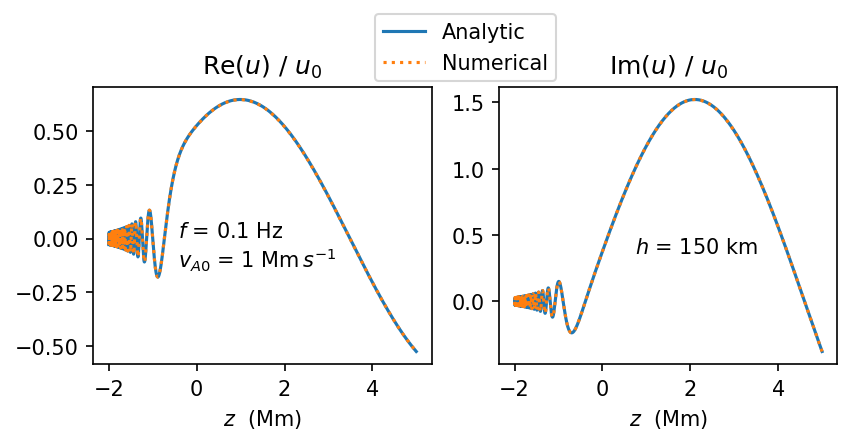
\includegraphics[width=\textwidth]{figures/chapter02/reflection_coefficent_u.png}
    \vspace{-20pt}
    \caption{This figure shows the real and imaginary parts of the normal mode velocity solution. The plots compare the solution calculated using Equation \eqref{eq:reflection_coefficent_u} with the solution calculated numerically. The parameters, $f$, $v_{A0}$, $h$, are listed as well. The code used to make this figure is available on GitHub in the following directory:\newline
    \href{https://github.com/aleksyprok/apkp_thesis/blob/main/Python/Chapter2/reflection_coefficent_u.py}{$\rightarrow$ Python/Chapter2/reflection\_coefficent\_u.py}}
    \vspace{-10pt}
    \label{fig:reflection_coefficent_u}
\end{figure}

In Figure \ref{fig:reflection_coefficent_u} we plot the real and imaginary components of $u$. It suggests that the solution given by Equation \eqref{eq:reflection_coefficent_u} is probably accurate as it agrees with the numerical solution. The numerical solution was calculated using a Runge-Kutta algorithm. More precisely, we used \texttt{solve\_ivp} from \citet{SciPy2020}. We initialised the code with the values of $u$ and $\dv*{u}{z}$ at $z=z_{min}$ using Equations \eqref{eq:reflection_coefficent_u} and \eqref{eq:reflection_coefficent_du_dz}. In the plots we let $h=150\si{.km}$, this value is used in for example \citet{Hollweg1984b}. Note that, if the mean mass of a molecule is given by $m_p/2$, $g_\odot$ is given by \eqref{eq:gravitational_acceleration} then from Equation \eqref{eq:pressure_scale_height} we know that
\[h \approx 151\si{.km}\qty(\frac{T}{10^4\si{.K}}).\]
We used a frequency of $f=0.1\si{.Hz}$, from Figure \ref{fig:power_spectrum_morton} we can see that this is on the high end of the observed frequencies.

\begin{figure}
    \centering
    \vspace{-20pt}
    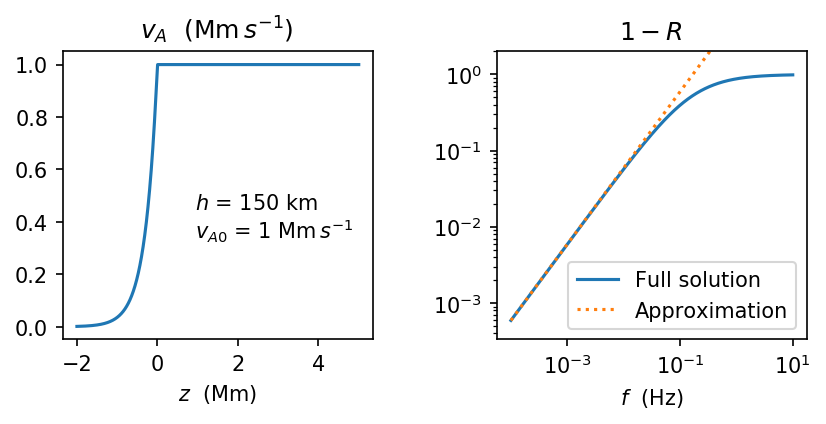
\includegraphics{figures/chapter02/reflection_coefficent.png}
    \vspace{-20pt}
    \caption{This figure shows 1 minus the reflection coefficient, $R$, (right) for the Alfv\'en speed shown on the left. We show the full solution in blue and the approximation, given by Equation \eqref{eq:reflection_coefficent_approximation}, is shown in dotted orange. The code used to make this figure is available on GitHub in the following directory:\newline
    \href{https://github.com/aleksyprok/apkp_thesis/blob/main/Python/Chapter2/reflection_coefficent_u.py}{$\rightarrow$ Python/Chapter2/reflection\_coefficent\_u.py}}
    \vspace{-10pt}
    \label{fig:reflection_coefficent}
\end{figure}

We are mainly interested in the reflection coefficient which we define as 
\begin{equation}
    R = \abs{\frac{c_4}{u_0}}.
\end{equation}
Note that
\begin{equation}
    \bar{H}_0^{(2)}(\xi_0) = H_0^{(1)}(\xi_0),
\end{equation}
and the Wronskian, $W\qty(H_0^{(1)},H_0^{(2)})(\xi)$, is given by
\begin{equation}
    W\qty(H_0^{(1)},H_0^{(2)})(\xi)=H_0^{(1)}H_0'^{(2)}-H_0'^{(1)}H_0^{(2)}=-\frac{4i}{\pi \xi}
\end{equation}
therefore,
\begin{equation}
    \begin{aligned}
        |c_4|^2 &= u_0^2\frac{\abs{H_0^{(2)}}^2 + \abs{H_1^{(2)}}^2 + i\qty(-H_0^{(2)}\bar{H}_1^{(2)}+ H_1^{(2)}\bar{H}_0^{(2)})}{\abs{H_0^{(2)}}^2 + \abs{H_1^{(2)}}^2 + i\qty(H_0^{(2)}\bar{H}_1^{(2)}- H_1^{(2)}\bar{H}_0^{(2)})} \\
        &= u_0^2\frac{\abs{H_0^{(2)}}^2 + \abs{H_1^{(2)}}^2 - 4/(\pi\xi_0)}{\abs{H_0^{(2)}}^2 + \abs{H_1^{(2)}}^2 + 4/(\pi\xi_0)}.
    \end{aligned}
\end{equation}
For typical values, $\xi_0$ is given by
\[\xi_0\approx0.57\times10^{-2}\qty(\frac{h}{150\si{.km}})\qty(\frac{\omega}{6\pi\times10^{-3}\si{.Hz}})\qty(\frac{1\si{.Mm.s^{-1}}}{v_{A0}}).\]
For $\xi_0\ll 1$, $R$ can be approximated as
\begin{equation}
    \label{eq:reflection_coefficent_approximation}
    R = 1 - \pi \xi_0 + O\qty(\xi_0^2).
\end{equation}
1 minus the reflection coefficient and its approximation are plotted in Figure \ref{fig:reflection_coefficent}. It shows that longer wavelength (or lower frequency) waves have larger reflection coefficients. If the wavelength of the wave is longer than the pressure scale height, $h$, then a large fraction of the wave energy will reflect at $z=0$. If the wavelength is shorter than $h$, the waves mostly leak out of the corona into the chromosphere and photosphere.

\section{Leaky loop: general solution}
\label{sec:leaky_loop_general_solution}

This section aims to calculate the general solution for a leaky loop, i.e. a loop where the boundaries' reflection coefficient is less than 1.

Since the loop is leaky, our system's boundary conditions can no longer be given by Equation \eqref{eq:bcs_chap_2}. To precisely define our boundary conditions we introduce a set of variables called Els\"asser variables $\mathcal{Z}^+$, $\mathcal{Z}^-$ which are defined as
\begin{equation}
    \label{eq:elsasser_z}
    \mathcal{Z}^\pm = u \pm v_{A0}\frac{b}{B_0}.
\end{equation}
From Equations \eqref{eq:uy_eqn_linear} and \eqref{eq:by_eqn_linear} we know that
\begin{equation}
    \begin{aligned}
    \pdv{u}{t} &= \frac{v_{A0}^2}{B_0}\pdv{b}{z}, \\
    \frac{v_{A0}}{B_0}\pdv{b}{t} &= v_{A0}\pdv{u}{z}.
    \end{aligned}
\end{equation}
Adding and subtracting the above equations gives
\begin{equation}
    \label{eq:elsasser_advection}
    \pdv{\mathcal{Z}^\pm}{t}\mp v_{A0}\pdv{\mathcal{Z}^\pm}{z}=0,
\end{equation}
respectively. Equation \eqref{eq:elsasser_advection} gives the 1D advection equation for negative propagating and positive propagating waves, respectively, where positive propagating waves travel in the positive $z$-direction. It shows that $\mathcal{Z}^+$ travels in the negative direction and $\mathcal{Z}^-$ travels in the positive direction. We define the boundary conditions as 
\begin{equation}
    \label{eq:bcs_elsasser}
    \begin{aligned}
    \mathcal{Z}^-(-l_z, t) &= 2f_{driv}(t) - R \mathcal{Z}^+(-l_z, t), \\
    \mathcal{Z}^+(l_z, t) &= -R \mathcal{Z}^-(l_z, t) \\
    \end{aligned}
\end{equation}
where $R$ is the reflection coefficient. Note that for $R=1$ we recover Equation \eqref{eq:bcs_chap_2} since $u = (\mathcal{Z}^+ + \mathcal{Z}^-) / 2$. The motivation for these boundary conditions is that each time a wave reaches $\pm l_z$ a fraction $R$ of the amplitude is reflected.

The full solution with the boundary conditions given by \eqref{eq:bcs_elsasser} and initial conditions given by \eqref{eq:initial_condition} is given by
\begin{equation}
    \label{eq:leaky_loop_general_solution}
    \begin{aligned}
    u(z,t) = \sum_{k=0}^m(-1)^kR^kH(\theta_k)f_{driv}(\theta_k),
    \end{aligned}
\end{equation}
where $\theta_k$ is given by Equation \eqref{eq:theta_k} and $m$ is given by Equation \eqref{eq:m} which for convenience we write again here
\begin{equation}
    \tag{\ref{eq:theta_k}}
    \theta_k=t-(-1)^k\frac{z}{v_{A0}}-\frac{(2k+1)l}{v_{A0}},
\end{equation}
\begin{equation}
    \tag{\ref{eq:m}}
    m = \left\lfloor\frac{t v_{A0}}{L_z}\right\rfloor.
\end{equation}
Note that this is almost the same as Equation \eqref{eq:closed_loop_general_solution_finite} except a factor $R^k$ has been introduced. From Equation \eqref{eq:by_eqn_linear} we know that $b$ is given by
\begin{equation}
    b(z,t) = -\frac{B_0}{v_{A0}}\sum_{k=0}^mR^kH(\theta_k)f_{driv}(\theta_k).
\end{equation}

\begin{figure}
    \centering
    \vspace{-20pt}
    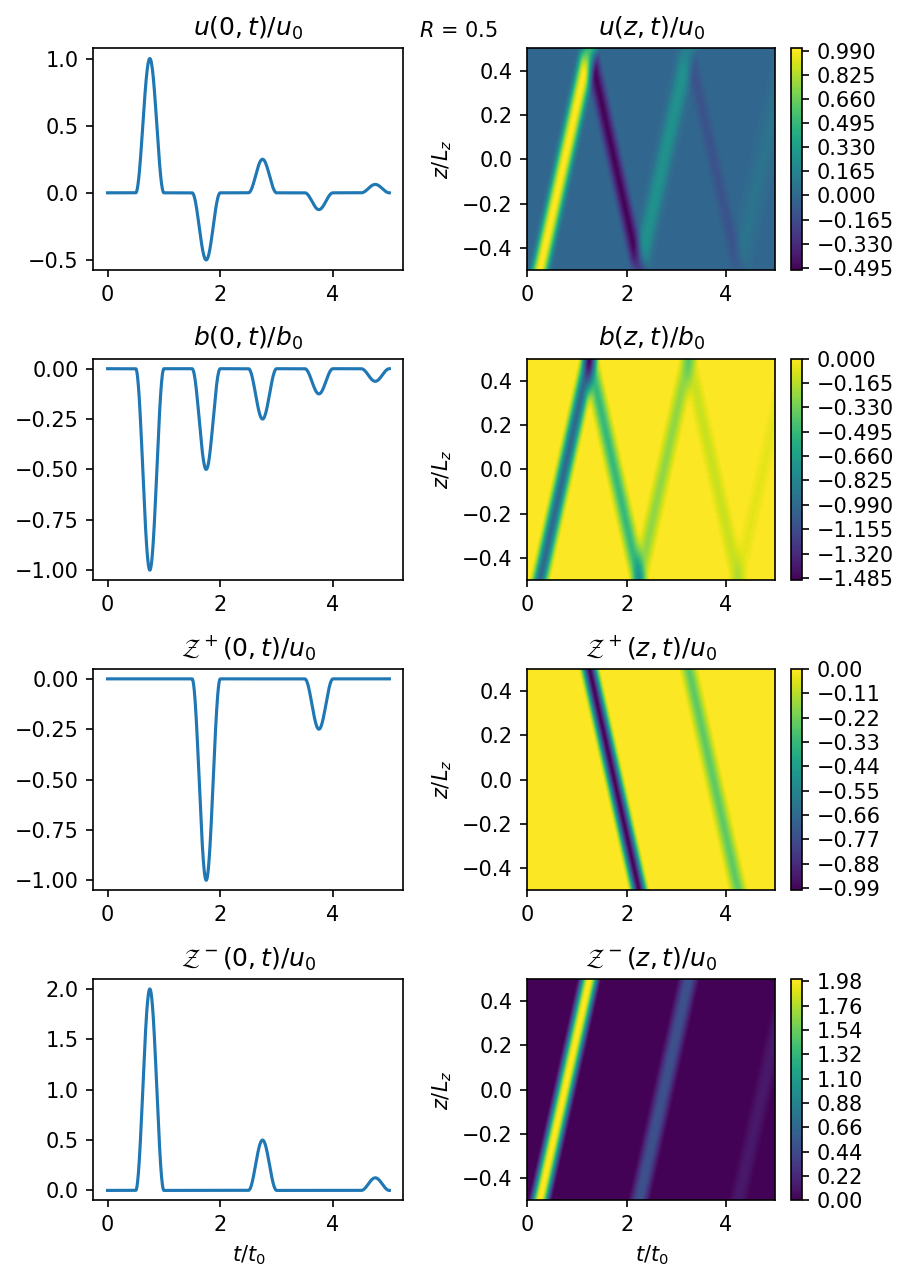
\includegraphics[width=\textwidth,height=0.9\textheight,keepaspectratio]{figures/chapter02/leaky_pulse.png}
    \vspace{-10pt}
    \caption{This figure plots $u$, $b$, $\mathcal{Z}^{+}$, $\mathcal{Z^{-}}$ for the case where $f_{driv}(t)$ is given by Equation \eqref{eq:f_driv_leaky_pulse} and this gives a pulse wave. Here the reflection coefficient is given by $R=0.5$. Note that $b_0$ is given by Equation \eqref{eq:b0}. The code used to make this figure is available on GitHub in the following directory:\newline
    \href{https://github.com/aleksyprok/apkp_thesis/blob/main/Python/Chapter2/leaky_pulse.py}{$\rightarrow$ Python/Chapter2/leaky\_pulse.py}}
    \vspace{-30pt}
    \label{fig:leaky_pulse}
\end{figure}

The solution is plotted in Figure \ref{fig:leaky_pulse} for the case where $f_{driv}$ produces a pulse. The driver is given by
\begin{equation}
    \label{eq:f_driv_leaky_pulse}
    f_{driv} = u_0\begin{cases}
    \sin^2(2\pi t / t_0), & t \le t_0 / 2,  \\
    0, & t > t_0 / 2,
    \end{cases}
\end{equation}
where $t_0$ is given by Equation \eqref{eq:t0}. The reflection coefficient is given by $R=0.5$. It shows that the wave's amplitude reduces by a factor $R$ each time it reflects at one of the boundaries. The figure confirms that $\mathcal{Z}^-$ does indeed correspond to positive propagating waves and $\mathcal{Z}^+$ corresponds to negative propagating waves.

\begin{figure}
    \centering
    \vspace{-20pt}
    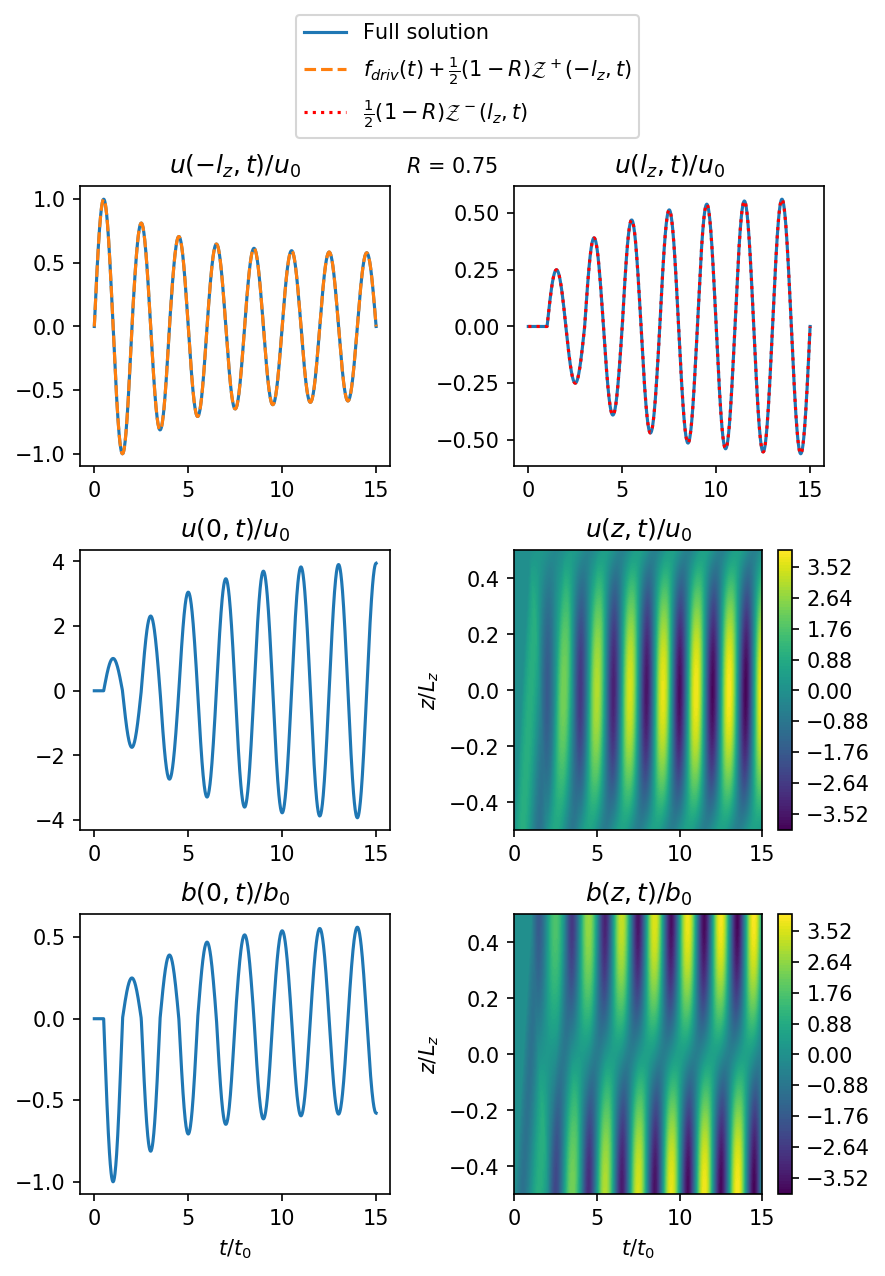
\includegraphics[width=\textwidth,height=0.85\textheight,keepaspectratio]{figures/chapter02/leaky_wave.png}
    \vspace{-10pt}
    \caption{This figure plots $u$, $b$, $\mathcal{Z}^{+}$, $\mathcal{Z^{-}}$ for the case where $f_{driv}(t)$ is given by Equation \eqref{eq:f_driv_leaky_wave} and this gives a continuous sinusoidal wave. Here the reflection coefficient is given by $R=0.75$. The top row show plots at $z=-l_z$ (left) and $z=l_z$ (right) and they show that the boundary conditions given by Equation \eqref{eq:bcs_elsasser} are satisfied. The code used to make this figure is available on GitHub in the following directory:\newline
    \href{https://github.com/aleksyprok/apkp_thesis/blob/main/Python/Chapter2/leaky_wave.py}{$\rightarrow$ Python/Chapter2/leaky\_wave.py}}
    \vspace{-30pt}
    \label{fig:leaky_wave}
\end{figure}

Figure \ref{fig:leaky_wave} plots the solution for the case where $f_{driv}$ produces a continuous sinusoidal wave. The driver is given by
\begin{equation}
    \label{eq:f_driv_leaky_wave}
    f_{driv} = u_0 \sin(\pi t / t_0).
\end{equation}
It confirms that the boundary conditions are satisfied since Equation \eqref{eq:bcs_elsasser} implies that
\begin{equation}
\begin{aligned}
    u(-l_z,t) &= f_{driv}(t)+\frac{1}{2}(1-R)\mathcal{Z}^+(-l_z,t) \\
    u(l_z,t) &= \frac{1}{2}(1-R)\mathcal{Z}^-(l_z,t). \\
\end{aligned}
\end{equation}
The plots also suggest that waves saturate at a maximum amplitude despite being driven at the resonant frequency for $R<1$. For $t\rightarrow \infty$ the amplitude of the waves saturates and the system oscillates at the driver frequency and we say it is at steady-state. The period in which the amplitude of the wave is changing is called the transient phase.

\section{Leaky loop: steady state solution}
\label{sec:leaky_loop_steady_state_solution}

At the end of the previous section, we suggested that for a continuous sinusoidal driver and $R<1$, the system will evolve towards a steady-state. At steady-state, the system oscillates at the driver frequency, and the amplitude saturates at a constant value. This section aims to prove that this is true for all frequencies and calculate the wave's amplitude at steady-state for a continuous sinusoidal driver.

Let $f_{driv}$ be given by
\begin{equation}
    \tag{\ref{eq:driver_sinusoidal}}
    f_{driv}(t)=u_0\exp(i\omega t).
\end{equation}
We seek the solution for $t \rightarrow\infty$, therefore, from Equation \eqref{eq:leaky_loop_general_solution}, we know that $u$ is given by
\[
    \begin{aligned}
    u(z,t) &= u_0\sum_{k=0}^\infty(-1)^kR^kH(\theta_k)\exp(i\omega\theta_k) \\
=&u_0\exp(i\omega[t-z/v_{A0}-l_z/v_{A0}])\frac{1}{2}\sum_{k=0}^{\infty}(1+(-1)^k)R^k\exp(-2i\omega l_z/v_{A0})^k-\\
&u_0\exp(i\omega[t+z/v_{A0}-l_z/v_{A0}])\frac{1}{2}\sum_{k=0}^{\infty}(1-(-1)^k)R^k\exp(-2i\omega l_z/v_{A0})^k. \\
    \end{aligned}
\]
Using the formula for an infinite geometric series the steady state solution is given by,
\begin{equation}
    \label{eq:leaky_steady_state_u}
    u(z,t) = u_0\exp(i\omega[t - l_z/v_{A0}])\frac{\exp(-i\omega z / v_{A0})-r\exp(i\omega z / v_{A0})}{1-r^2},
\end{equation}
provided $R<1$, where
\begin{equation}
    \label{eq:lower_case_r}
    r = R\exp(-2i\omega l_z / v_{A0}).
\end{equation}
Using Equation \eqref{eq:by_eqn_linear} the magnetic field is given by
\begin{equation}
    \label{eq:leaky_steady_state_b}
    b= -\frac{B_0u_0}{v_{A0}}\exp(i\omega[t - l_z/v_{A0}])\frac{\exp(-i\omega z / v_{A0})+r\exp(i\omega z / v_{A0})}{1-r^2}
\end{equation}

\begin{figure}
    \centering
    \vspace{-20pt}
    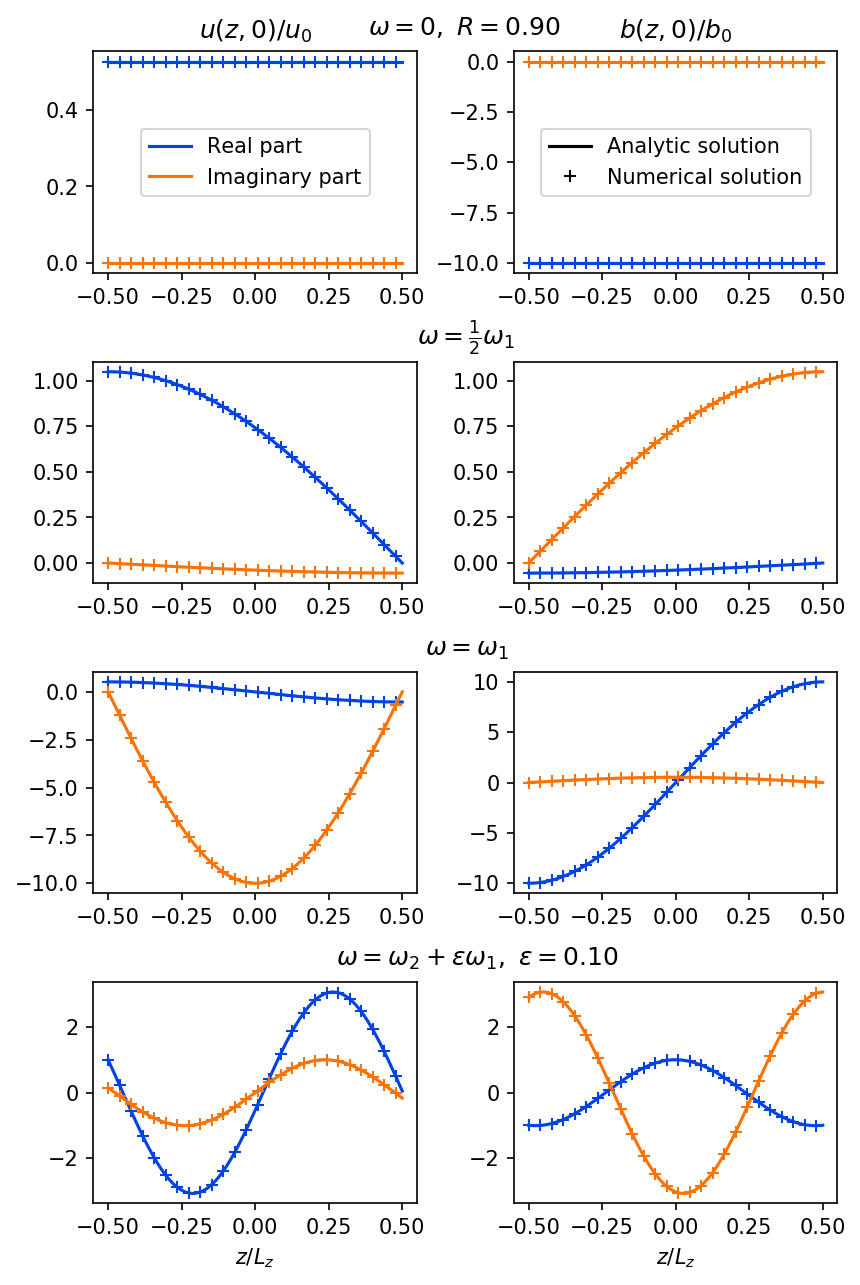
\includegraphics[width=\textwidth,height=0.85\textheight,keepaspectratio]{figures/chapter02/steady_state_soln_along_z.png}
    \vspace{-10pt}
    \caption{This figure shows plots of the steady state velocity (left) and magnetic field (right) along $z$. In each row a different frequency driver is used. The analytic solutions (solid line) were calculated using Equations \eqref{eq:leaky_steady_state_u} and \eqref{eq:leaky_steady_state_b}. The numerical solutions (+ symbols) were calculated by solving the boundary value problem described by Equation \eqref{eq:numerical_elssasser_eqn} using \texttt{solve\_bvp} in \citet{SciPy2020}. The code used to make this figure is available on GitHub in the following directory:\newline
    \href{https://github.com/aleksyprok/apkp_thesis/blob/main/Python/Chapter2/steady_state_soln.py}{$\rightarrow$ Python/Chapter2/steady\_state\_soln.py}}
    \vspace{-30pt}
    \label{fig:steady_state_soln_along_z}
\end{figure}

We can also calculate the steady-state solution via a numerical approach. This is useful to check that the analytic solution is correct. We seek the steady-state solution where the whole system oscillates at the driver frequency. Therefore, we can assume that the time dependence is given by $\exp(i\omega t)$. Assuming the time dependence implicitly, we can simplify the PDEs given by Equation \eqref{eq:elsasser_advection} into the following ODEs,
\begin{equation}
    \label{eq:numerical_elssasser_eqn}
    \dv{Z^{\pm}}{z}=\pm i\frac{\omega}{v_{A0}}Z^{\pm}.
\end{equation}
Note that this system of ODEs is coupled due to the boundary conditions given by Equation \eqref{eq:bcs_elsasser}. We can solve this boundary value problem numerically using \texttt{solve\_bvp} in \citet{SciPy2020}. In Figure \ref{fig:steady_state_soln_along_z} we plot the real and imaginary parts of the steady state velocity, $u$, and magnetic field, $b$ as a function of $z$ at $t=0$. For each plot $R=0.9$. The top-row plots the solution for $\omega=0$. The second row plots the solution for $\omega=\omega_1/2$, where $\omega_1$ is the fundamental resonant frequency, see Equation \eqref{eq:chap_2_omega_n}. The third row plots the solution for $\omega = \omega_1$. Finally, the last row plots the solution for $\omega=\omega_2 + 0.1\omega_1$. They show that the numerical and analytic solutions agree and this suggests that Equations \eqref{eq:leaky_steady_state_u} and \eqref{eq:leaky_steady_state_b} are accurate.

\begin{figure}
    \centering
    \vspace{-20pt}
    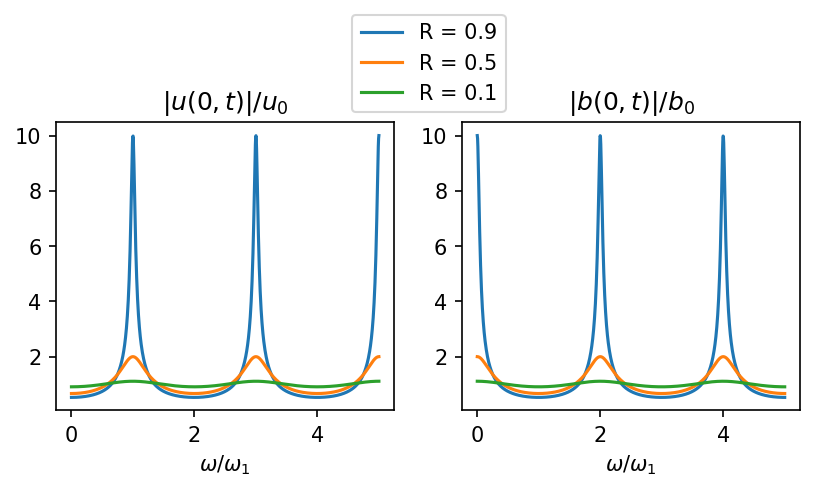
\includegraphics[width=\textwidth,height=0.9\textheight,keepaspectratio]{figures/chapter02/steady_state_soln_at_z=0.png}
    \vspace{-30pt}
    \caption{This figure shows plots of the absolute value of the velocity and magnetic field at $z=0$ as a function of the driver frequency, $\omega$, for $R=0.9$, 0.5 and 0.1. The absolute values were calculated using Equations \eqref{eq:abs_leaky_steady_state_u} and \eqref{eq:abs_leaky_steady_state_b}. Note that $b_0$ is given by Equation \eqref{eq:b0}. The code used to make this figure is available on GitHub in the following directory:\newline
    \href{https://github.com/aleksyprok/apkp_thesis/blob/main/Python/Chapter2/steady_state_soln_at_z\%3D0.py}{$\rightarrow$ Python/Chapter2/steady\_state\_soln\_at\_z=0.py}}
    \label{fig:steady_state_soln_at_z=0}
\end{figure}

At $z=0$, Equation \eqref{eq:leaky_steady_state_u} can be simplified to give
\begin{equation}
    \label{eq:leaky_steady_state_u_z=0}
    u(0,t) = u_0\exp(i\omega[t - l_z/v_{A0}])\frac{1}{1+r},
\end{equation}
and Equation \eqref{eq:leaky_steady_state_b} gives
\begin{equation}
    \label{eq:leaky_steady_state_b_z=0}
    b(0,t) = -\frac{B_0u_0}{v_{A0}}\exp(i\omega[t - l_z/v_{A0}])\frac{1}{1-r}.
\end{equation}
Therefore, the absolute value of $u(0,t)$ is given by
\begin{equation}
    \label{eq:abs_leaky_steady_state_u}
    \abs{u(0,t)} = \frac{u_0}{\sqrt{R^2+2R\cos(2\omega l_z / v_{A0})+1}},
\end{equation}
and the absolute value of $b(0,t)$ is given by
\begin{equation}
    \label{eq:abs_leaky_steady_state_b}
    \abs{b(0,t)} = \frac{B_0 u_0 / v_{A0}}{\sqrt{R^2-2R\cos(2\omega l_z / v_{A0})+1}}.
\end{equation}
In Figure \ref{fig:steady_state_soln_at_z=0} we use Equations \eqref{eq:abs_leaky_steady_state_u} and \eqref{eq:abs_leaky_steady_state_b} to plot the absolute value of the steady state  velocity, $u$ and magnetic field $b$ at $z=0$ as function of the driver frequency, $\omega$. The values are shown for $R=0.9$, 0.5 and 0.1. It shows that as $R\rightarrow 1$ then the absolute value goes to infinity at the resonant frequencies.

\section{Open loop: phase mixing}
\label{sec:phase_mixing}

This chapter has modelled the plasma as ideal, i.e. we have neglected resistivity and viscosity. We justify this because the Reynolds numbers for observed wavelengths is much greater than unity, see Equations \eqref{eq:visc_reynolds_number} and \eqref{eq:mag_reynolds_number}. This section introduces a mechanism, namely phase mixing, that can generate very short length-scales, resulting in very small Reynolds numbers. Phase mixing is the process where gradients perpendicular to the field build-up due to Alfv\'en waves propagating on field lines with a spatial gradient in Alfvén travel time. Where the Alfv\'en travel time is the time it takes for Alfv\'en waves to propagate along the loop over a given distance. To illustrate phase mixing, we calculate the time evolution of driven Alfv\'en waves propagating in an open domain where $v_A=v_A(x)$.

We introduce an $x$-dependence, i.e. let
\[u = u(x,z,t),\quad b = b(x,z,t),\quad v_{A0} = v_A(x).\]
Note that the magnetic field is still given by Equation \eqref{eq:background_field}.
We impose a driver at $z=0$ and impose open boundary conditions. Hence, $\mathcal{Z}^+=0$, i.e. the solution can only contain solutions propagating in the positive $z$-direction. Therefore, $u=\mathcal{Z}^-/2$, and substituting this into Equation \eqref{eq:elsasser_advection} gives
\begin{equation}
    \label{eq:advection_positive}
    \pdv{u}{t}+v_A(x)\pdv{u}{z}=0.
\end{equation}
We aim to solve Equation \eqref{eq:advection_positive} with the following initial condition
\begin{equation}
    u(x,z,0) = 0,
\end{equation}
and boundary condition
\begin{equation}
    u(x,0,t) = f_{driv}(x,t).
\end{equation}
This has the solution
\begin{equation}
    u(x,z,t) = H\qty(t - \frac{z}{v_A(x)})f_{driv}\qty(x,t - \frac{z}{v_A(x)}).
\end{equation}

Consider the case where
\begin{equation}
    f_{driv}(x, t) = u_0\sin(\omega t),
\end{equation}
and
\begin{equation}
    v_A(x) = v_{A0}\qty(1+\frac{x}{L_x}),
\end{equation}
where $x > -L_x$.
Hence,
\begin{equation}
    u(x,z,t) = u_0H\qty(t - \frac{z}{v_A(x)})\sin\qty[\omega\qty(t - \frac{z}{v_A(x)})].
\end{equation}

\begin{figure}
    \centering
    \vspace{-20pt}
    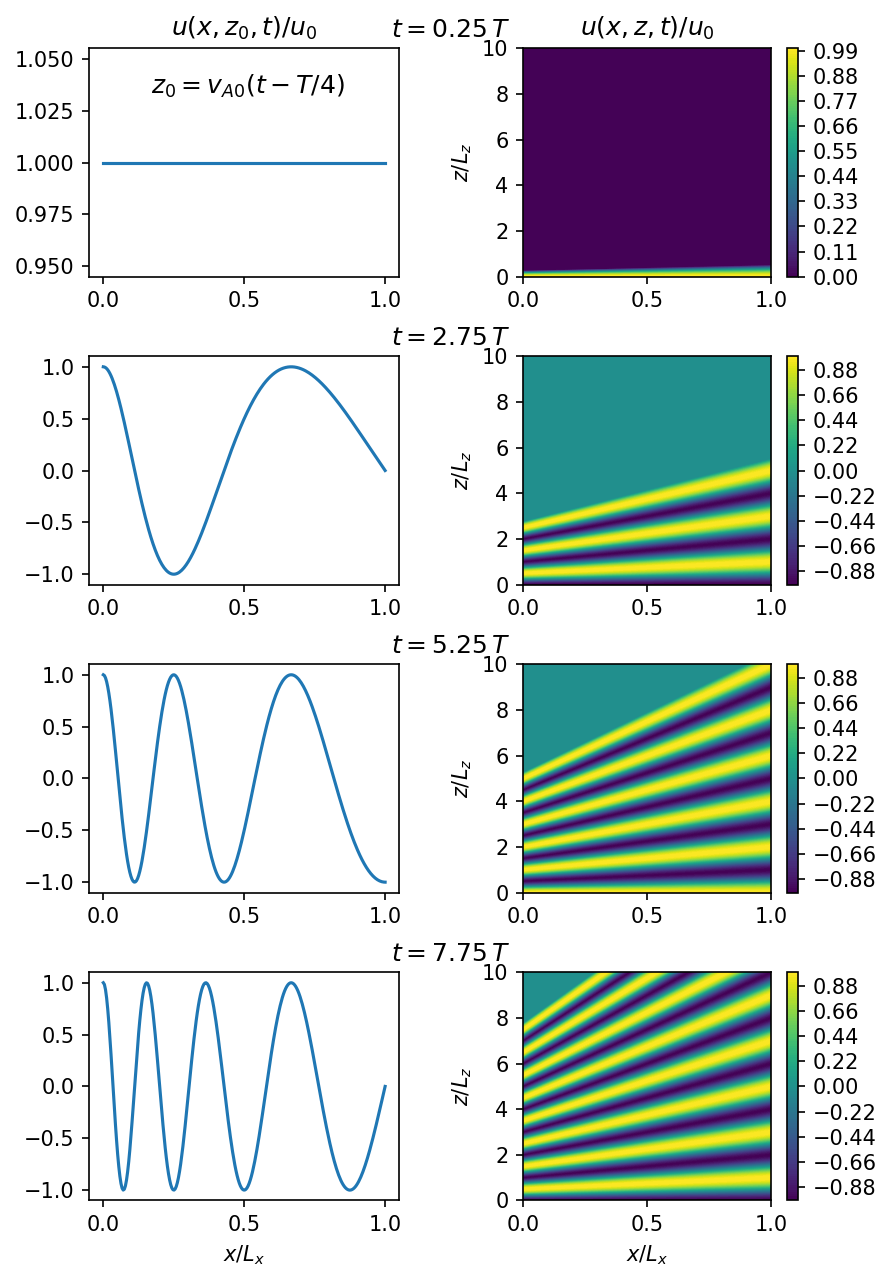
\includegraphics[width=\textwidth,height=0.85\textheight,keepaspectratio]{figures/chapter02/phase_mixing.png}
    \vspace{-10pt}
    \caption{This figure shows snapshots of the velocity, where each row corresponds to a different time. The left side plots the velocity as a function of $x$ at $z=z_0$, where $z_0$ is given by the expression in the top-left plot. The right side shows a contour plot of the velocity as a function of $x$ and $z$. The code used to make this figure is available on GitHub in the following directory:\newline
    \href{https://github.com/aleksyprok/apkp_thesis/blob/main/Python/Chapter2/phase_mixing.py}{$\rightarrow$ Python/Chapter2/phase\_mixing.py}}
    \vspace{-30pt}
    \label{fig:chap_2_phase_mixing}
\end{figure}

We plot this solution in Figure \ref{fig:chap_2_phase_mixing}. It shows the velocity at different snapshots. Note that in Figure \ref{fig:chap_2_phase_mixing}
\[T=\frac{2\pi}{\omega},\ L_z = \frac{2\pi}{\omega}v_{A0}.\]
The top row shows the solution at $t=T/4$, the second row is at $t = 11T/4$, the third row is at $t = 21 T/4$ and the bottom row is at $t = 31 T/4$. The left side shows plots along $x$ at $z=z_0$ where $z_0$ is given by
\[z_0 = v_{A0}\qty(t - \frac{T}{4}).\]
The right side shows contour plots of the velocity as a function of $x$ and $z$. They show that the length-scale in $x$ gets shorter as the wave propagates further along. Consider the plots on the left side, the top plot is equal to a constant value in $x$, we think of this as a curve with only one peak, the second plot has two peaks, the third plot has three peaks, and the bottom plot has four peaks. To quantify the rate at which the length-scales decrease, consider the following.
Assume, $t>z/v_A(x)$, hence,
\begin{equation}
    u(x,z,t) = u_0\sin\qty[\omega\qty(t - \frac{z}{v_A(x)})].
\end{equation}
Taking the $x$-derivative gives
\begin{equation}
    \label{eq:phase_mixing_du_dx}
    \pdv{u}{x} = u_0\omega \dv{v_A}{x}\frac{z}{v_A^2}\cos\qty[\omega\qty(t - \frac{z}{v_A(x)})].
\end{equation}
This shows that the gradients in $x$ grow linearly with $z$.

\section{Discussion and conclusions}

In this chapter, our goal was to introduce some key properties of ideal footpoint driven Alfv\'en waves relevant for the rest of this thesis. In Section \ref{sec:chap_2_closed_loop_general_soln} we showed how d'Alambert's formula and a method of images approach can be used to calculate the general solution in a closed loop. In Section \ref{sec:closed_loop_sinusoidal_solution} we showed that if the driver is of the form $\exp(i\omega t)$ then the general solution can be simplified using the geometric series formula. We showed that if the driving frequency is equal to one of the natural frequencies, i.e. $\omega = \omega_n$, (where $\omega_n$ is given by Equation \ref{eq:chap_2_omega_n}), then the energy of the solution will grow quadratically and ubounded in time. If $\omega\ne\omega_n$ then the solution will oscillate about a finite value. We showed in Figures \ref{fig:case_where_omega=omega_n_u} and \ref{fig:case_where_omega=omega_n_b} that if the driver frequency equals the the zeroth harmonic, $\omega=\omega_0=0$, then then only the magnetic energy grows to infinity and the kinetic energy oscillates about a finite value. Whereas, for the other harmonics, i.e. $\omega_n$ for $n\ge1$, both the kinetic and magnetic kinetic energy grows to infinity. If $\omega=\omega_0$ then the velocity of the driver never changes sign, which stretches the magnetic field, resulting in a large build-up of magnetic energy for a small amount of kinetic energy. If $\omega=\omega_n$ for $n\ge 1$ then a standing wave is set up and this has approximately equal magnetic and kinetic energy (averaged over one wave period).

The sinusoidal driver is useful because it is relatively easy to calculate the exact solution. In reality, the photosphere will excite a range of frequencies, and this can be modelled by superimposing sinusoidal solutions via a Fourier series approach. In Section \ref{sec:closed_loop_random_driver} we calculate the solution for a broadband driver, i.e. a driver which excites a broad range of frequencies. In Section \ref{sec:chap_2_driven_harmonic_oscillator} we assumed a Fourier series solution in $z$ to convert the Alfv\'en wave equation, a PDE, into a set of ODEs for a driven harmonic oscillator. We calculated the exact solution for a red noise force and white noise force driver (in Section \ref{sec:noisy_force}, we define red and white noise). We also estimated the solutions with a red and white noise force driver by approximating them with a finite Fourier series. Figure \ref{fig:noisy_driver} compares the exact and approximate solutions and show they converge as the number of harmonics increases. The error shows a steep reduction if the resonant harmonic is excited. Note that red and white noise force drivers are unphysical because they have an infinite variance. However, they are still useful concepts because it is simple to calculate an exact analytic solution using a red and white noise force driver (see Section \ref{sec:noisy_force}). Moreover, the approximate solutions in Figure \ref{fig:noisy_driver} have a finite variance and show similar results. Results from Section \ref{sec:closed_loop_random_driver} show that the variance and energy grow linearly when either a red noise or white noise force driver is used. Whereas in Section \ref{sec:closed_loop_sinusoidal_solution} we showed that if a sinusoidal driver is used with $\omega=\omega_n$, the energy grows quadratically with time.

In Sections \ref{sec:chap_2_closed_loop_general_soln}-\ref{sec:closed_loop_random_driver} we used line-tied boundary conditions. These boundary conditions are motivated by the fact that the chromosphere is significantly denser than the corona. However, despite the large change in density, a small fraction of the waves will leak from the corona into the chromosphere. In Section \ref{sec:leaky_loop_reflection_coefficent} we calculate an estimate for the reflection coefficient using a similar model to that used in \citet{Hollweg1984b}. Figure \ref{fig:reflection_coefficent_u} plots the reflection coefficent as a function of frequency. It shows that the higher the frequency (i.e. shorter wavelength), the more the waves leak out of the corona. In Section \ref{sec:leaky_loop_general_solution} we calculate the general solution for waves in a leaky loop. We show that the solution evolves towards a state where the whole system oscillates at the driver frequency, and this is called the steady-state solution. In Section \ref{sec:leaky_loop_steady_state_solution} for a sinusoidal driver and confirm it numerically in Figure \ref{fig:steady_state_soln_along_z}. Figure \ref{fig:steady_state_soln_at_z=0} shows that the steady-state solution's amplitude is largest at the resonant frequencies and tends to infinity as the reflection coefficient, $R$, goes to 1. Note that the timescale to reach steady-state also grows to infinity as $R\rightarrow 1$, and so we recover the closed-loop solution as $R\rightarrow 1$.

Finally, in Section \ref{sec:phase_mixing} we introduce a phenomenon called phase mixing. Figure \ref{fig:chap_2_phase_mixing} shows if neighbouring field lines have different Alfv\'en speeds, this can result in Alfv\'en waves moving out of phase with their neighbours as they evolve. This results in the growth of steep gradients perpendicular to the field, which may be important in coronal heating, we discuss this further in the next chapter.

% To prove that the velocity is continuous we first show that the tangential component of the electric field, $\vec{E}$, is continuous. We apply Stokes' theorem to Faraday's law, Equation \eqref{eq:faradays_law}, to give the integral form of Faraday's law,
% \[\oint_{\partial S}\vec{E}\cdot d\vec{l} = -\int_S \pdv{\vec{B}}{t}\cdot d\vec{S}.\]
% We choose $S$ as a small rectangle across the interface. This is is illustrated in Figure \ref{fig:curl_e}. The sides perpendicular to the interface have length $h$ above and below the interface. The sides parallel to the interface have length l. Let $h\rightarrow0$, now the area of integration looks like a line, which as zero area. In other words,
% \[\lim_{h\rightarrow 0}\vec{S}=0.\]
% Since $\pdv*{\vec{B}}{t}$ remains finite in this limit, the whole right hand side goes to zero. All that is left is
% \[\oint_{\partial S}\vec{E}\cdot d\vec{l}=0.\]
% Assuming our rectangle is small enough that $E$ is roughly constant, its magnitude can be pulled out of the integral. As the remaining sides to our original rectangle, the $d\vec{l}$ in each region run in opposite directions, so we define one of them as the tangent unit vector, $\vec{t}$, and the other as $-\vec{t}$.
% Let the region $z<0$ be labelled medium 1 and the region $z>0$ be denoted medium 2. Hence,
% \[\vec{E}_2\cdot\vec{t}l-(\vec{E}_1\cdot\vec{t})l=0,\]
% \[\implies (\vec{E}_2-\vec{E}_1)\cdot\vec{t}=0.\]
% Therefore, we have proven that the tangential component of the electric field must be continuous across $z=0$.

% \begin{figure}
%     \centering
%     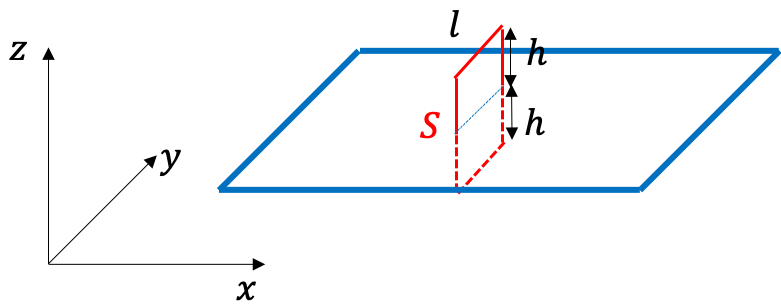
\includegraphics{figures/chapter02/curl_e.png}
%     \caption{This figure illustrates the rectangle, $S$, which is used to prove that the tangential component of the electric field is zero.}
%     \label{fig:curl_e}
% \end{figure}